% Version 0.2
\documentclass[a4paper]{article}
 
\usepackage[english,german]{babel}
\usepackage[utf8]{inputenc}
\usepackage[T1]{fontenc}
\usepackage{ae}
\usepackage{comment}
\usepackage[bookmarks,bookmarksnumbered]{hyperref}
\usepackage{enumerate}
\usepackage{datetime}
\usepackage[table,xcdraw]{xcolor}
\usepackage{graphicx}
\usepackage{longtable}

\DeclareGraphicsExtensions{.pdf,.png,.jpg,.jpeg,.gif}
\newcommand{\horrule}[1]{\rule{\linewidth}{#1}} % Create horizontal rule command with 1 argument of height

\author{Gruppe 17}

\title{
	\normalfont
	\normalsize 
	\huge{Pflichtenheft Buchhandlung Schiller}
	\horrule{0.5pt}
	\paragraph{Version: 0.4}
	\paragraph{Status: in Arbeit}
	\paragraph{Stand: \today}
	\horrule{2pt}
}

\begin{document}

\maketitle

\newpage
 
\section*{Zusammenfassung}

\paragraph{Dies ist das Pflichtenheft für das Projekt Buchhandlung Schiller. Dieses Projekt wird durch die Gruppe 17 betreut. Es handelt sich um eine Verkaufsanwendung, welche in Java programmiert wird, Diese Verkaufsanwendung stellt einen Internetauftritt als auch einen Onlineshop für die Buchhandlung Schiller dar. In diesem Pflichtenheft werden die Anforderungen an das Projekt festgeschrieben.}
 
\section*{Historie}

\begin{comment}

|l|l|l|l|l|

\end{comment}

\begin{tabular}{|r|r|c|l|c|}
	\hline
	\rowcolor[HTML]{C0C0C0} 
	Version & Status    & Datum      & Bearbeiter       & Erläuterung    	\\ \hline
	0.1     & In Arbeit & 30.10.2014 & Christoph Kepler & Initial Commit 	\\ \hline
	0.2     & In Arbeit & 01.11.2014 & Christoph Kepler & Diagramme      	\\ \hline
	0.3     & In Arbeit & 07.11.2014 & Christoph Kepler & Letzte Punkte  	\\ \hline
	0.4		& In Arbeit & 09.11.2014 & Christoph Kepler	& \LaTeX			\\ \hline
\end{tabular}

\section*{Reviewnachweis}

\begin{tabular}{|l|l|l|l|}
	\hline
	\rowcolor[HTML]{C0C0C0} 
	Version & Datum      & Reviewer       & Erläuterung    \\ \hline
\end{tabular}

\newpage

% Platzierung des Inhaltsverzeichnisses

\tableofcontents

\newpage
 
\section{Aufgabenstellung und Zielsetzung}

\paragraph{Die Buchhandlung SCHILLER benötigt eine Verkaufsanwendung. Hauptsächlich ist eine Verkaufsanwendung für die Bücher zu implementieren. Jedoch hat der Geschäftsführer noch einige eigene Ideen. 
Die Anwendung benötigt, neben einer Artikelverwaltung auch eine Benutzerverwaltung. Zu jedem Buch muss mindestens der Autor, Verlag, die ISBN und eine kurze Inhaltsbeschreibung gespeichert werden. Eine Abbildung des Buchbundes anzuzeigen, würde die Attraktivität des Verkaufsprogrammes deutlich steigern. Die Bücher der Buchhandlung SCHILLER sind nach Genre in die Kategorien Fiktion, Sachbuch, Unterhaltung, Ratgeber unterteilt. Eine Möglichkeit zu Erweiterung und nachträglichem Hinzufügen weiterer Genres ist wünschenswert. Der Geschäftsinhaber denkt auch über ein Angebot von CDs und DVDs nach. Die Benutzerverwaltung soll einige wichtige Angaben zum Kunden liefern (Name, Kundennummer, Lieferadresse, etc.). 
Als zusätzliches Feature wünscht der Buchhandel SCHILLER sich einen Kalender auf der Homepage, welcher die wöchentlichen Lesungen aufführt, die in den Räumen der Buchhandlung stattfinden. Die Bezahlung der gekauften Bücher erfolgt über Rechnungsversand.}

\section{Fachlicher Überblick}

\paragraph{Um die Aufgabenstellung zu realisieren wird das Java Framework Spring verwendet. Um die Verkaufsaspekte abzudecken, wird zusätzlich das Java Framework Salespoint eingesetzt. Diese beiden Frameworks sollen durch Wiederverwendung den Programmieraufwand so gering wie möglich halten. Die im SWT-Modul gelernten Design-Patterns sollen genutzt werden, um größtmögliche Modularisierung, einfache Erweiterbarkeit und unkomplizierte Wartung zu gewährleisten.}

\paragraph{Die zu erstellende Web Applikation stellt eine Verkaufsanwendung für die Buchandlung SCHILLER dar. Über diese Anwendung sollen Artikel in verschiedenen Kategorien zum Verkauf angeboten werden. Dazu müssen sich die Gäste an dem System mit ihrer korrekten E-Mail-Adresse registrieren. Es werden Rollen auf die einzelnen Nutzer verteilt, welche dadurch spezielle Berechtigungen auf das System erben. Für die verschiedenen Rollen ist es dann möglich ihrer Tätigkeit nach zu gehen. So kann zum Beispiel der Reading Manager die Lesungen in den dafür bereitgestellten Kalender und die Ressource Raum eintragen, solange nicht schon eine Lesung dort vorhanden ist. Der Rechnungsversand erfolgt automatisch als pdf via E-Mail an den Kunden.}

\section{Systemgrenze und Top-Level-Architektur}

\subsection{Kontextdiagramm}

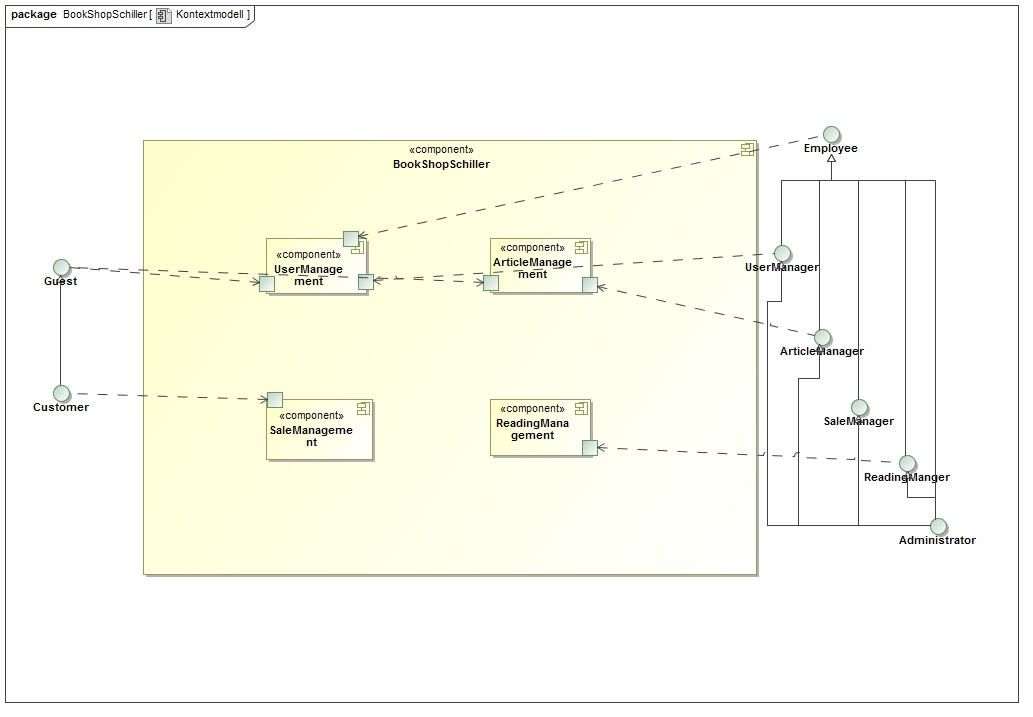
\includegraphics[width=350px]{kontextmodell.jpg}

\subsection{Top-Level-Architektur}

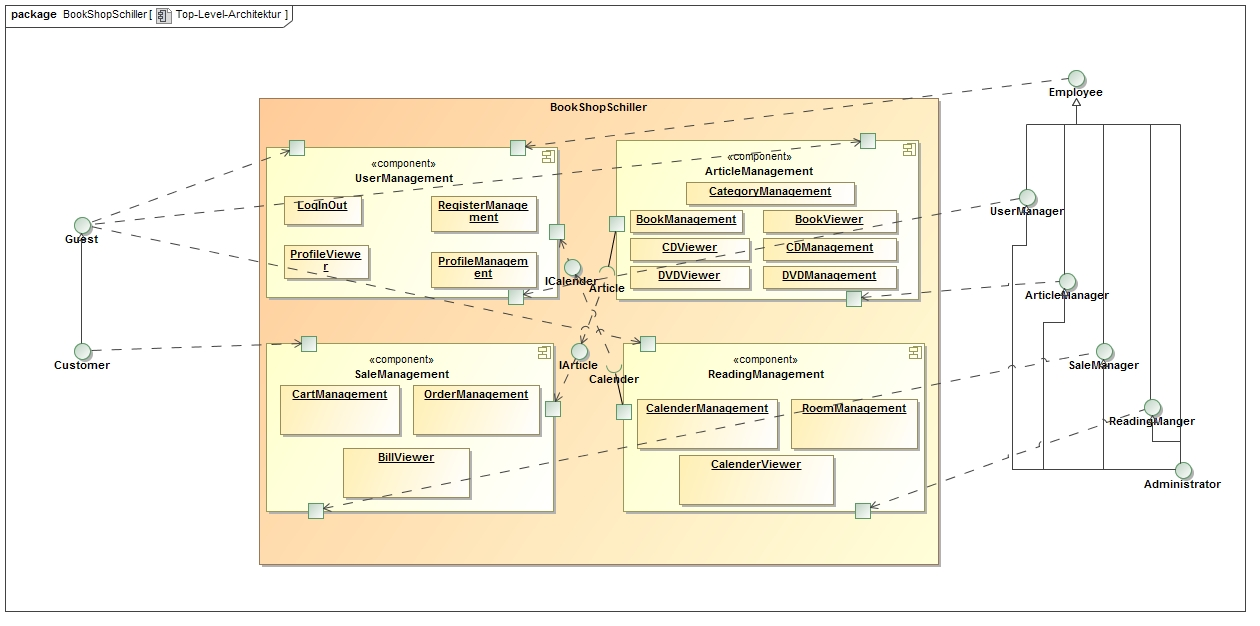
\includegraphics[width=350px]{top-level-architektur.jpg}

\section{Anwendungsfälle}

\subsection{Überblick: Anwendungsfalldiagramm}

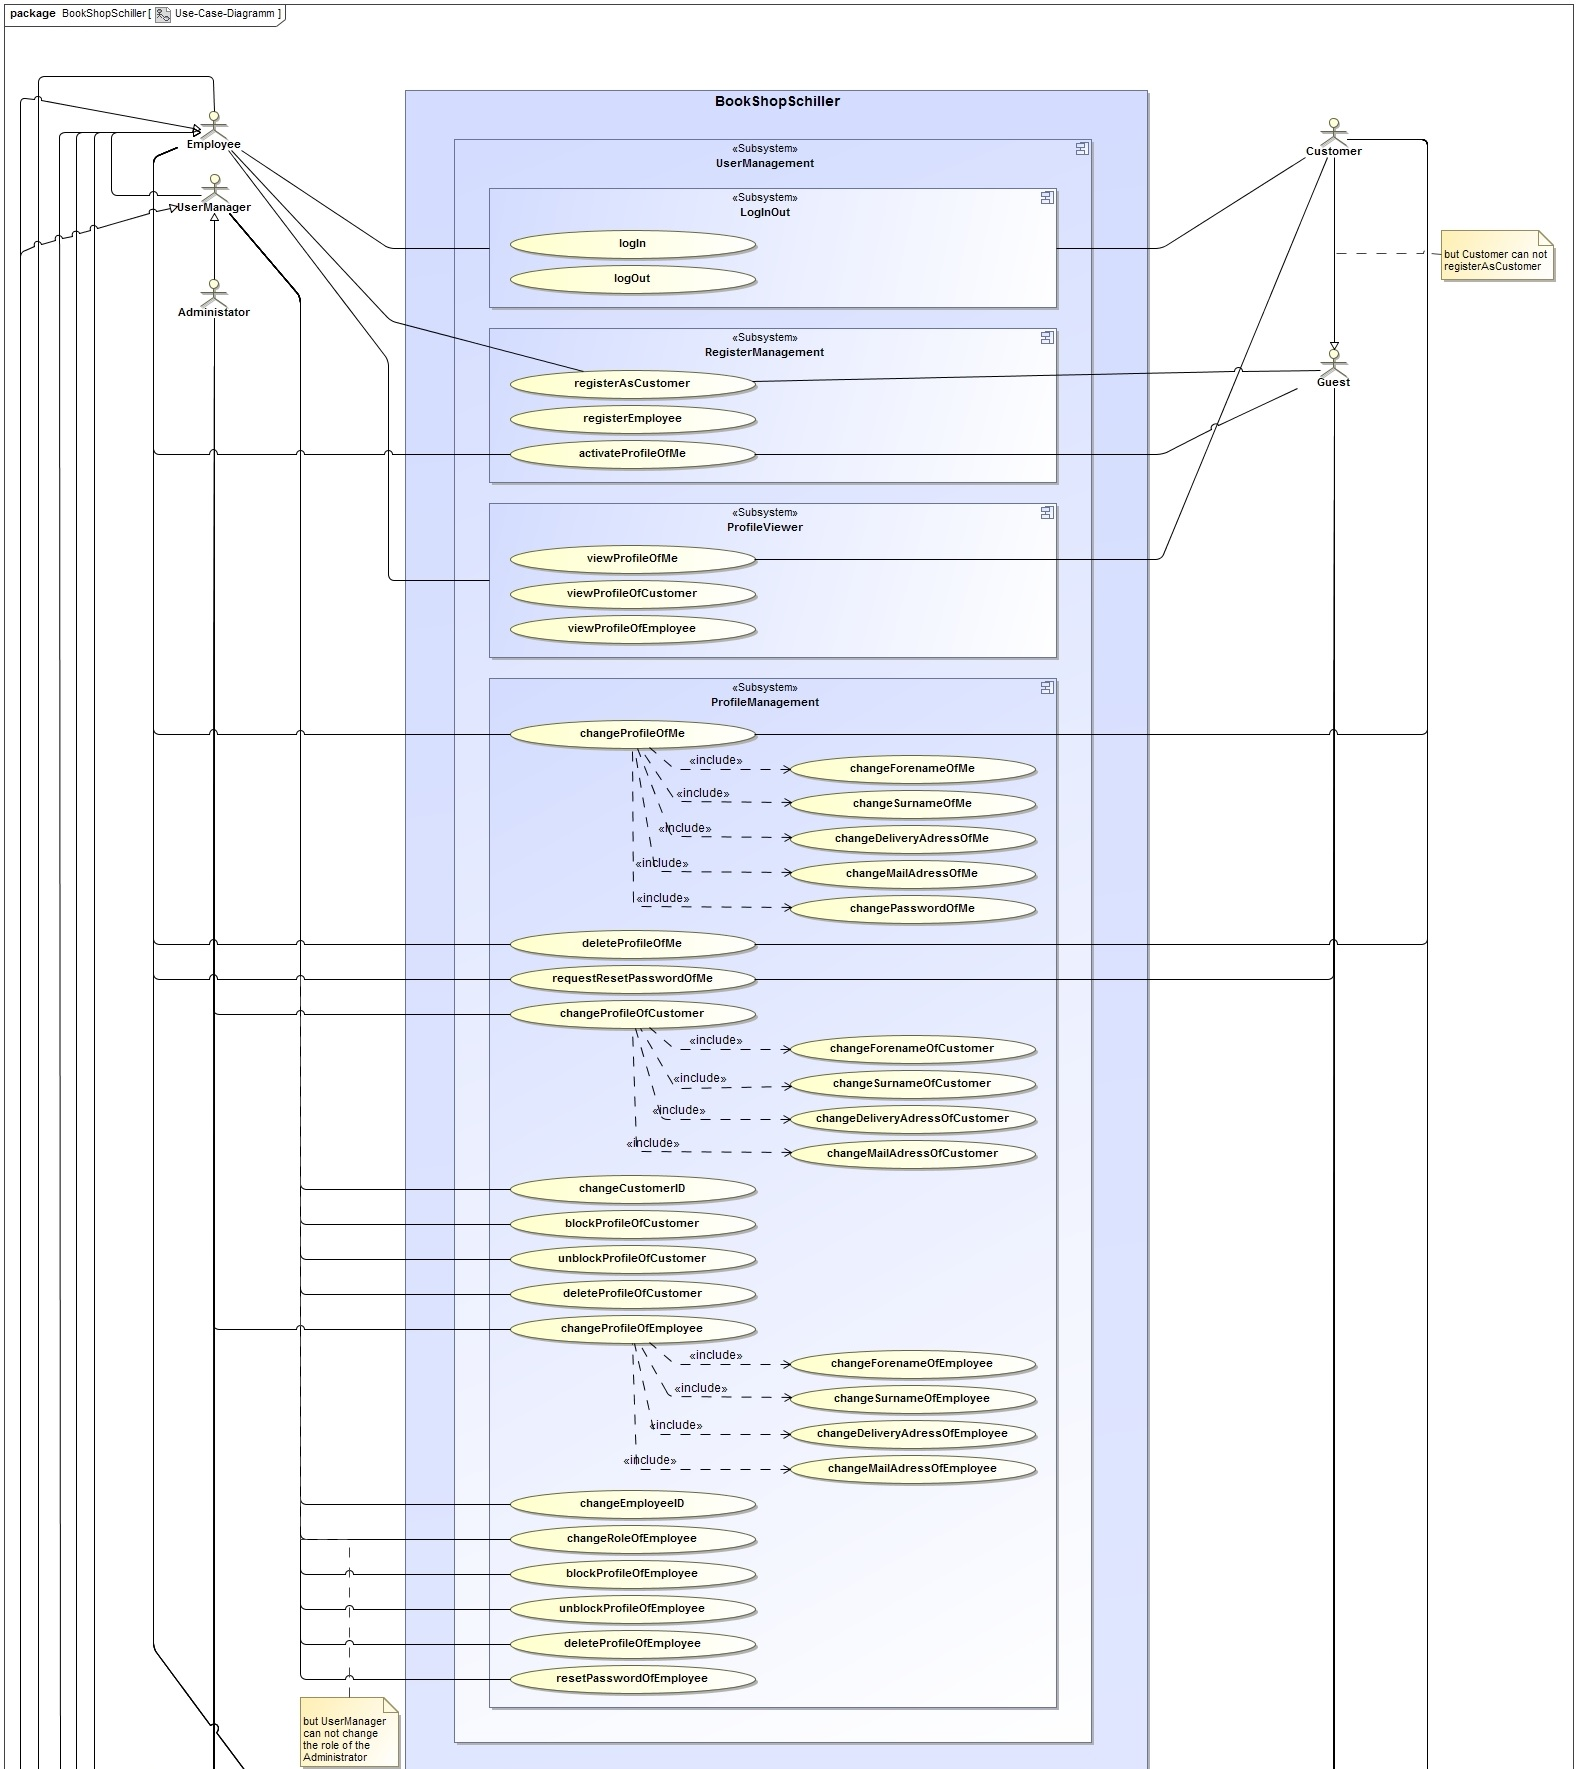
\includegraphics[width=350px]{use-case-diagramm-part1.jpg}

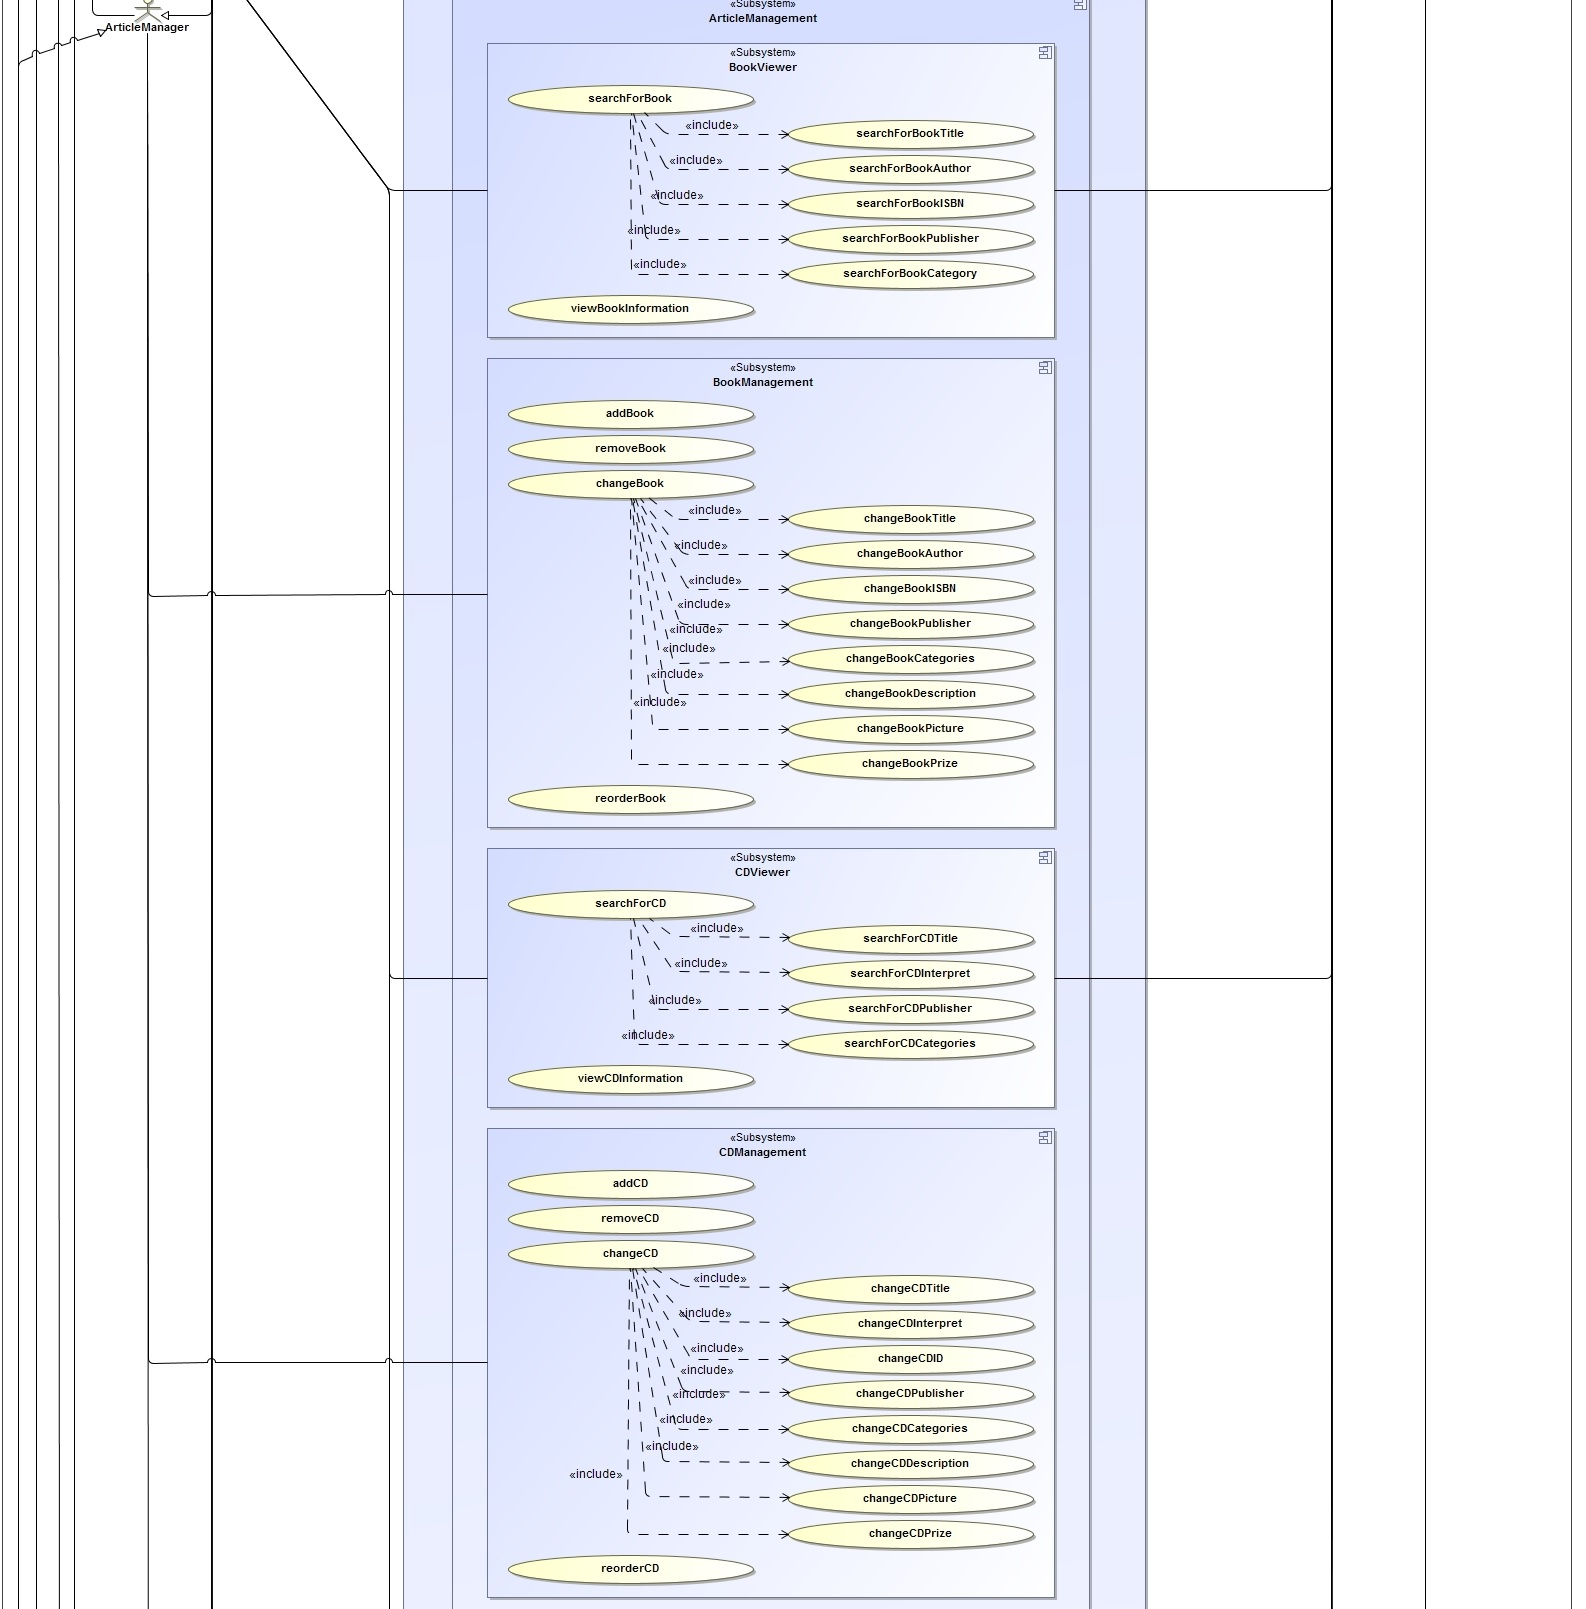
\includegraphics[width=350px]{use-case-diagramm-part2.jpg}

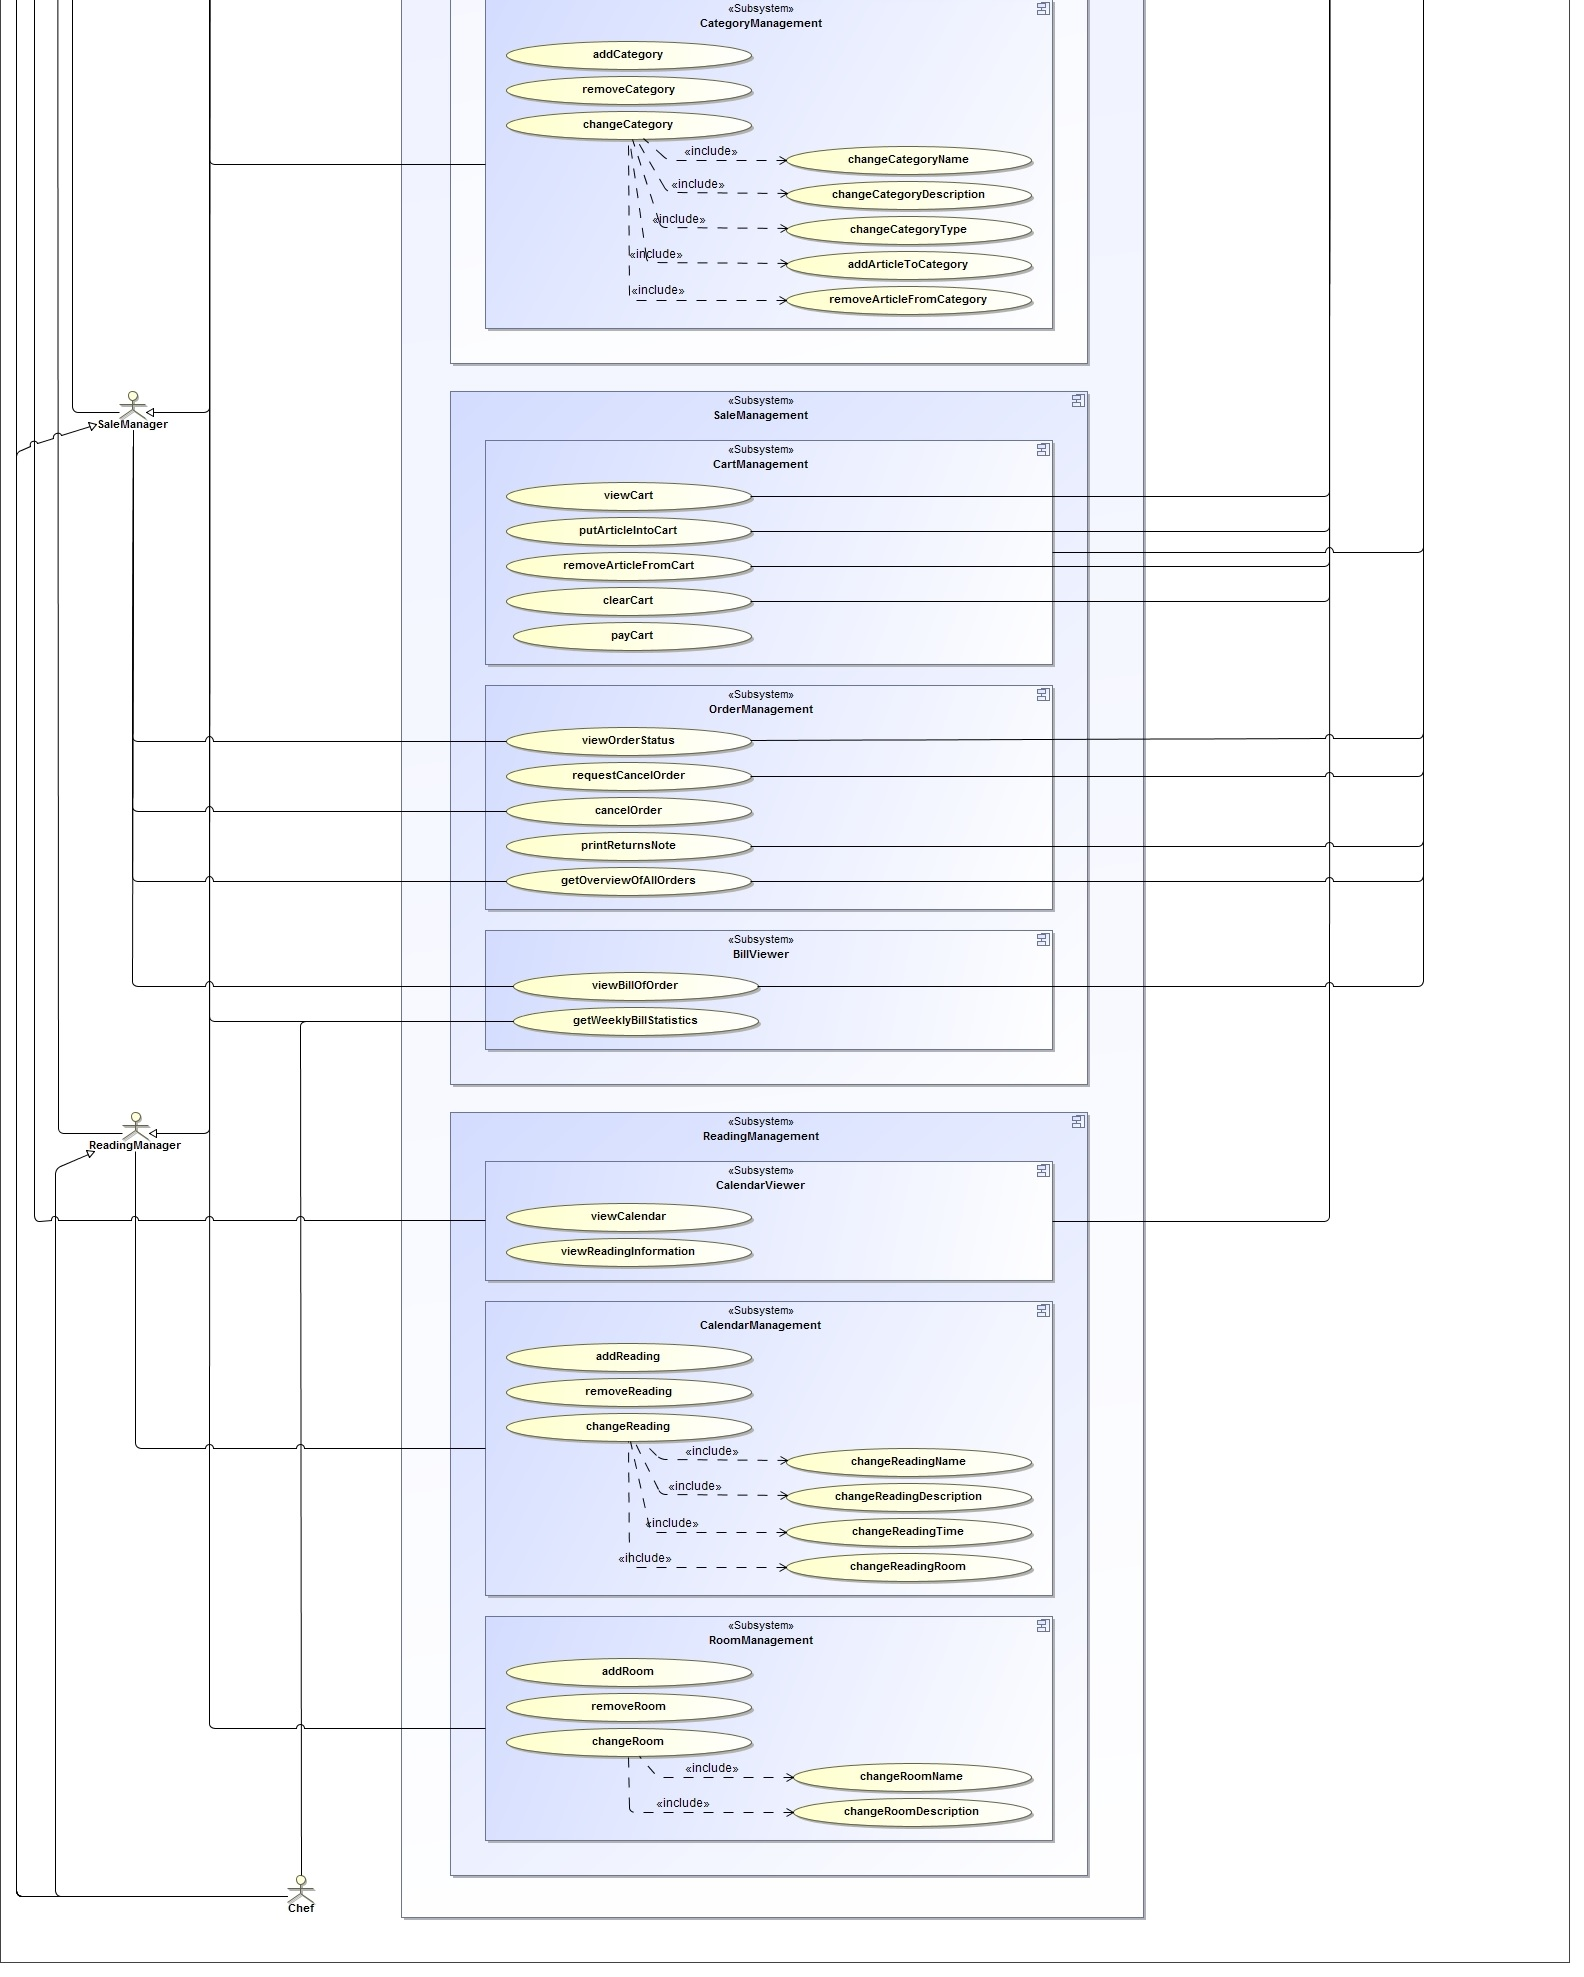
\includegraphics[width=350px]{use-case-diagramm-part3.jpg}

\subsection{Akteure}

\begin{tabular}{|p{100px}|p{250px}|}
	\hline
	\rowcolor[HTML]{C0C0C0} 
	Name & Beschreibung	\\ \hline
	Guest & Der Guest ist ein unauthentifizierter Nutzer der Anwendung.\\ \hline
	Customer & Der Customer ist ein authentifizierter Nutzer der Anwendung.\\ \hline
	Employee & Der Employee ist ein MitarbKlasse stellt die Umsetzung einer Kategorie dar.eiter der Firma.\\ \hline
	User Manager & Der User Manager ist der Verwalter von registrierten Nutzern im System.\\ \hline
	Article Manager & Der Article Manager ist der Verwalter vom Artikelbestand im System.\\ \hline
	Reading Manager & Der Reading Manager ist der Verwalter der Lesungen im System.\\ \hline
	Chef & Der Chef stellt den Chef der Firma da.\\ \hline
	Admin/Root/User 0 & Der Admin ist der Nutzer mit allen Rechten.\\ \hline
\end{tabular}

\subsection{Anwendungsfallbeschreibung}

\begin{longtable}{|p{100px}|p{250px}|}
	\hline
	\rowcolor[HTML]{C0C0C0}
	Use Case ID & Beschreibung \\ \hline
	\multicolumn{2}{|l|}{Usermanagement:}  \\ \hline
	UC01 & Login/Logout  \\ \hline
	UC02 & Register as user  \\ \hline
	\multicolumn{2}{|l|}{Userdata:} \\ \hline
	UC03 & different role management  \\ \hline
	UC04 & Manipulate  \\ \hline
	UC05 & View own  \\ \hline
	UC06 & View costumer  \\ \hline
	UC07 & Reset Password  \\ \hline
	\multicolumn{2}{|l|}{Article Management:}  \\ \hline
	UC08 & View Articles (Books, CD, DVD)  \\ \hline
	UC09 & Search articles via different criteria  \\ \hline
	UC10 & manipulate article inventory  \\ \hline
	UC11 & manipulate categories  \\ \hline
	\multicolumn{2}{|l|}{Sales Management:}  \\ \hline
	\multicolumn{2}{|l|}{Cart Management:}  \\ \hline
	UC12 & fill/empty cart  \\ \hline
	UC13 & checkout  \\ \hline
	\multicolumn{2}{|l|}{Order Management:}  \\ \hline
	UC14 & view order  \\ \hline
	UC15 & cancel/ get return  \\ \hline
	\multicolumn{2}{|l|}{Bill Management:}  \\ \hline
	UC16 & view \\ \hline
	UC17 & statistics \\ \hline
	\multicolumn{2}{|l|}{Reading Management:} \\ \hline
	UC18 & view/ manipulate calender \\ \hline
	UC19 & manipulate reading events \\ \hline
	UC20 & manipulate rooms \\ \hline
\end{longtable}

\begin{comment}
\begin{itemize}
	\item[\textbf{Usermanagement:}]
	\item Login/Logout
	\item Register as user
	\item[\textbf{Userdata:}]
	\item different role management
	\item Manipulate
	\item View own
	\item View costumer
	\item Reset Password
	\item[\textbf{Article Management:}]
	\item View Articles (Books, CD, DVD)
	\item Search articles via different criteria
	\item manipulate article inventory
	\item manipulate categories
	\item[\textbf{Sales Management:}]
	\item
	\begin{itemize}
		\item[\textbf{Cart Management:}]
		\item fill/empty cart
		\item checkout
		\item[\textbf{Order Management:}]
		\item view order
		\item cancel/ get return
		\item[\textbf{Bill Management:}]
		\item view
		\item statistics
	\end{itemize}
	\item[\textbf{Reading Management:}]
	\item view/ manipulate calender
	\item manipulate reading events
	\item manipulate rooms
\end{itemize}
\end{comment}

\section{Sequenzdiagramme}

\subsection{Article Management}

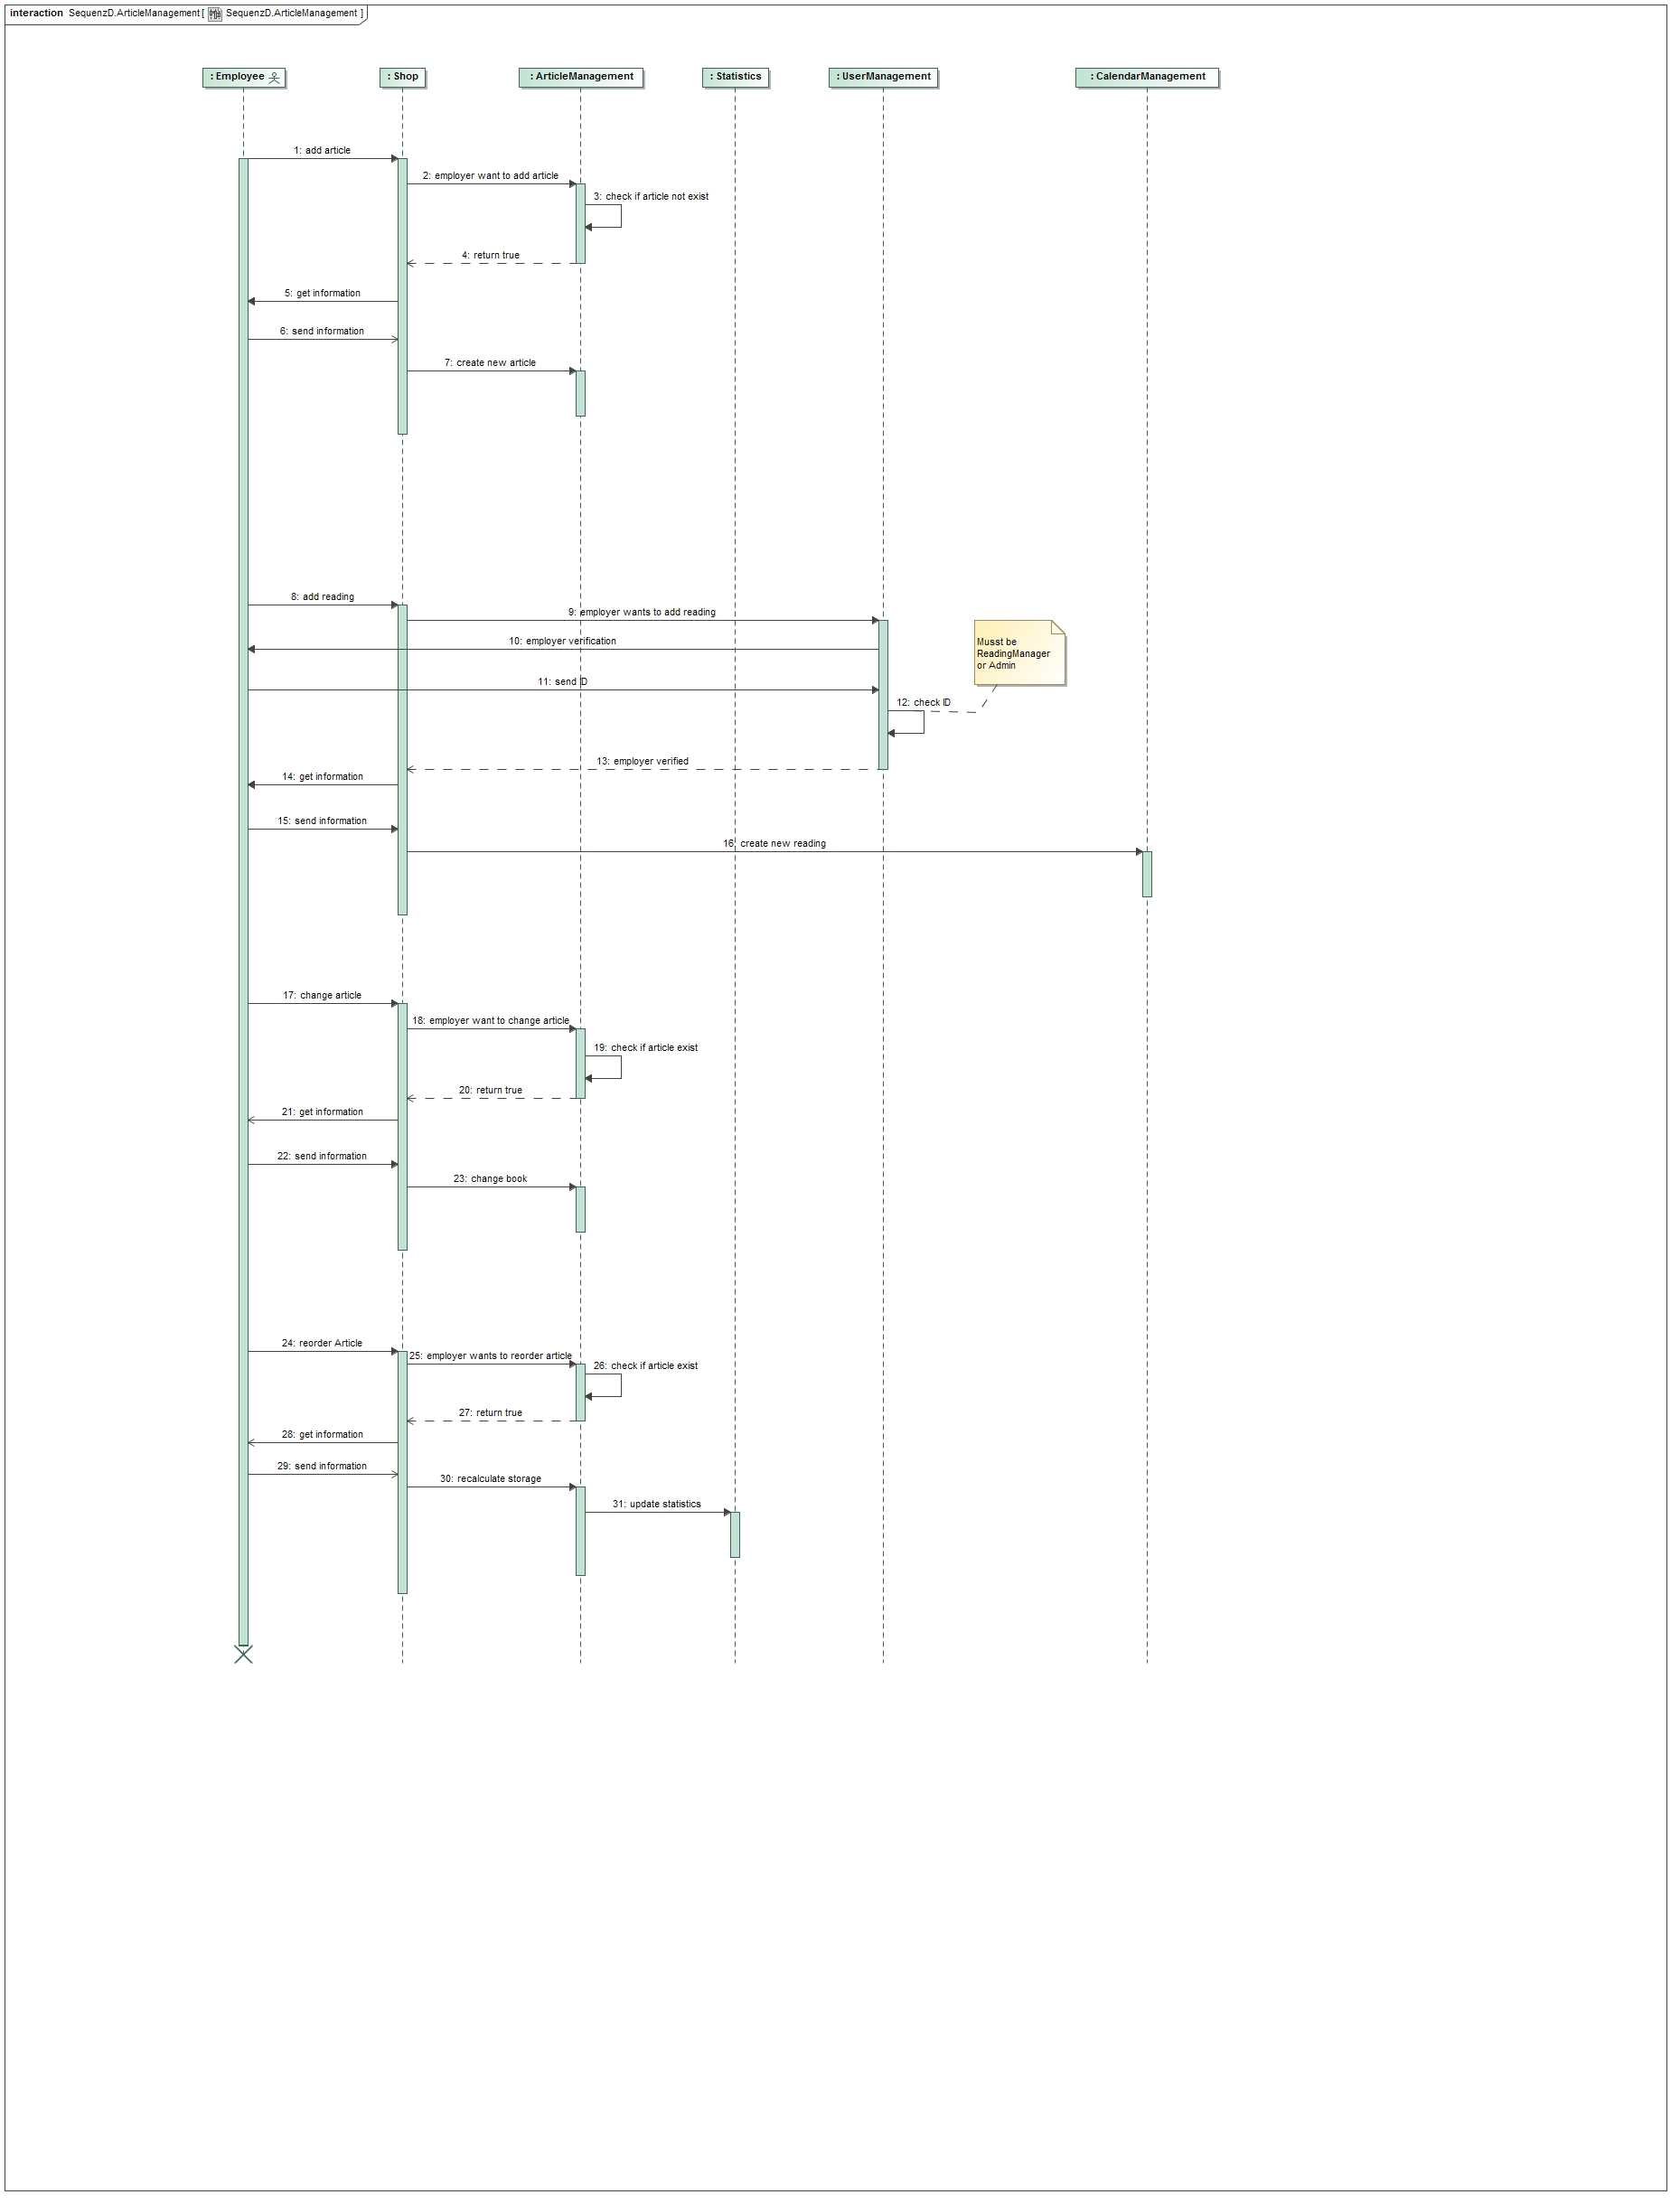
\includegraphics[width=350px]{sd-articlemanagement.jpg}

\subsection{Profile Management}

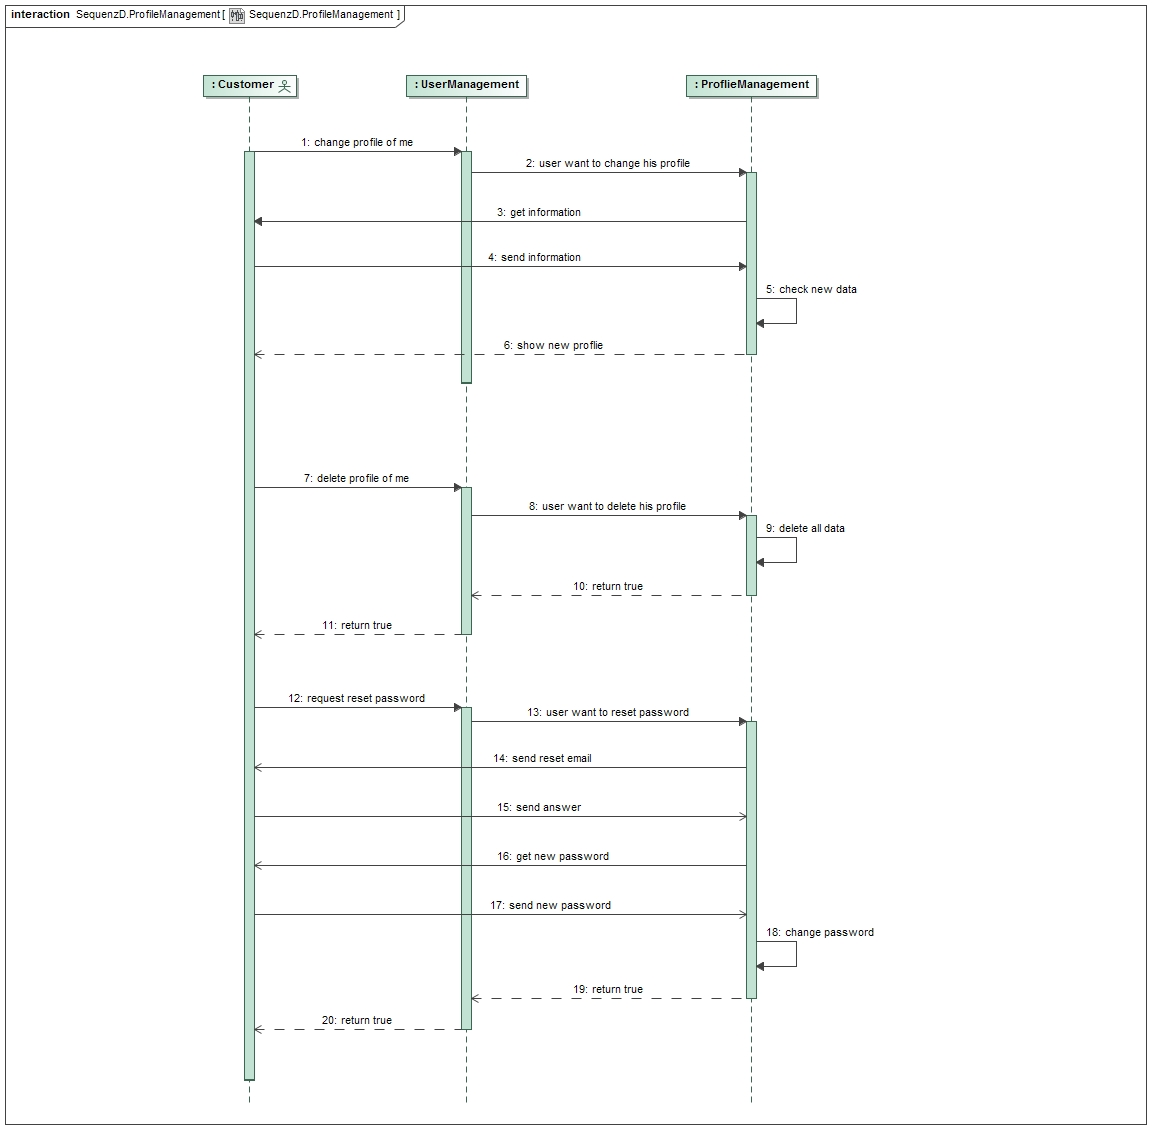
\includegraphics[width=350px]{sd-profilemanagement.jpg}

\subsection{Purchase}

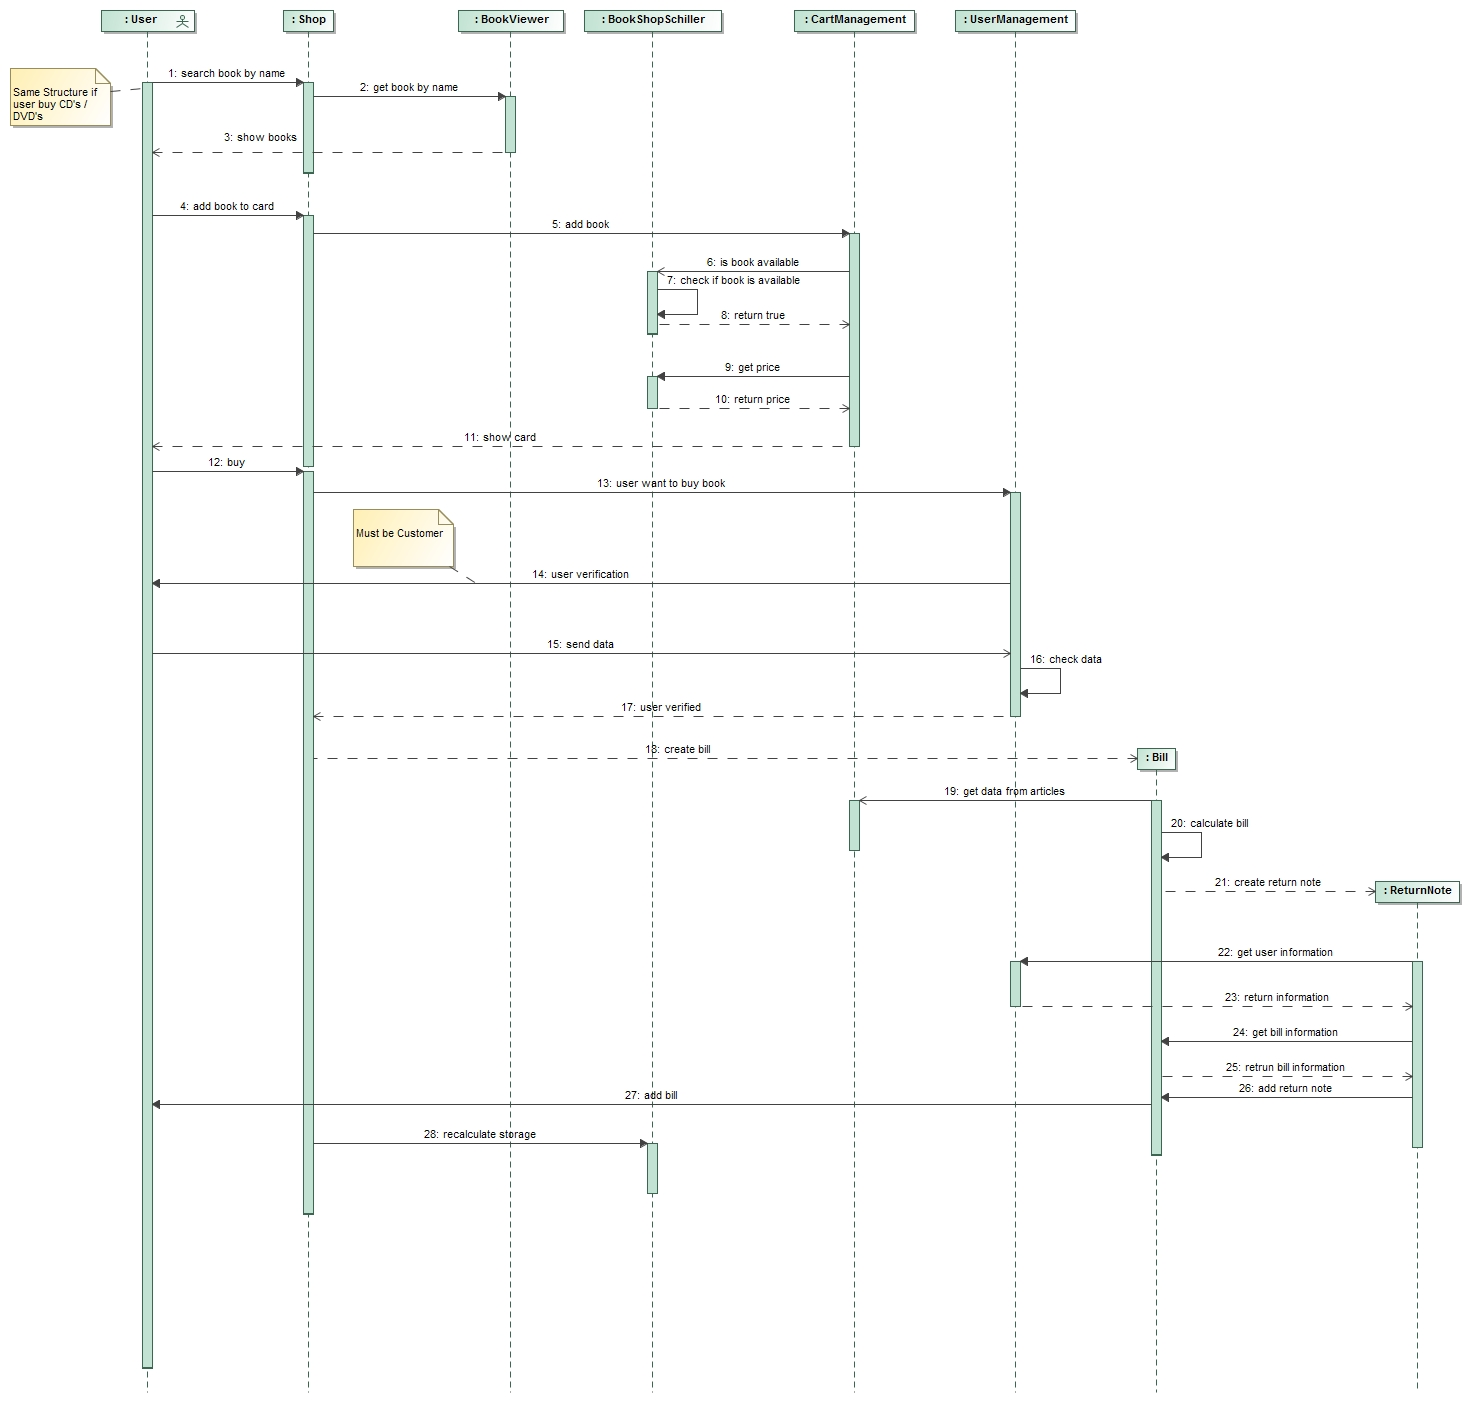
\includegraphics[width=350px]{sd-purchase.jpg}

\subsection{Registration}

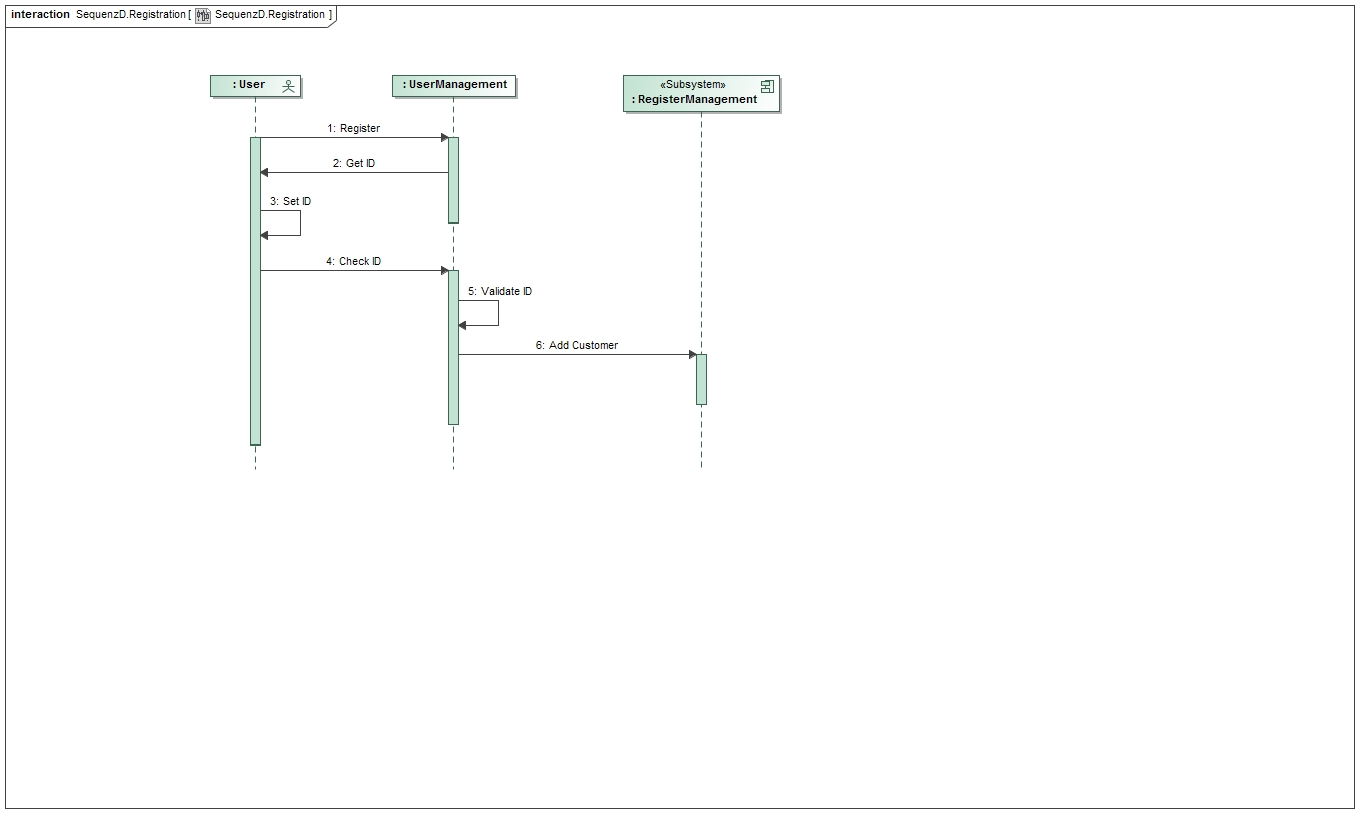
\includegraphics[width=350px]{sd-registration.jpg}

\section{Anforderungen}

\subsection{Musskriterien}

\begin{longtable}{|p{100px}|p{250px}|}
	\hline
	\rowcolor[HTML]{C0C0C0}
	Criteria ID & Beschreibung \\ \hline
	CUM01 & Akteure: Mitarbeiter, nicht eingeloggter Nutzer, eingeloggter Nutzer, Chef, Administrator, Personalverwalter \\ \hline
	CUM02 & Nutzeraccount kann mehrere Rollen haben \\ \hline
	CUM03 & mind. ein Root im System  \\ \hline
	CAM01 & artikelspezifische Kategorien  \\ \hline
	CCM01 & Kalender für wöchentliche Lesungen  \\ \hline
	\multicolumn{2}{|l|}{Guest kann:} \\ \hline
	CAM02 & Artikel suchen \\ \hline
	CCM02 & Artikel in Warenkorb legen \\ \hline
	CSM01 & nicht kaufen \\ \hline
	\multicolumn{2}{|l|}{Customer kann:} \\ \hline
	CSM02 & kaufen \\ \hline
	CSM03 & Übersicht über bereits gekaufte Artikel anzeigen \\ \hline
	CBM01 & Rechnung online anzeigen lassen und herunterladen \\ \hline
	\multicolumn{2}{|l|}{Employee kann:} \\ \hline
	CAM03 & Artikelbestand sehen \\ \hline
	CAM04 & ggf. nachbestellen \\ \hline
	\multicolumn{2}{|l|}{User Manager kann:} \\ \hline
	CUM04 & Rollen der anderen Nutzer verändern, außer Root \\ \hline
	\multicolumn{2}{|l|}{Chef kann:]} \\ \hline
	CSM04 & wöchentliche Verkaufsbilanzen anzeigen \\ \hline
	\multicolumn{2}{|l|}{Root kann:} \\ \hline
	CUM05 & alles \\ \hline
	CAM05 & Kategorien manipulieren \\ \hline
	CRM01 & Räume manipulieren \\ \hline
\end{longtable}

\begin{comment}
\begin{itemize}
	\item Akteure: Mitarbeiter, nicht eingeloggter Nutzer, eingeloggter Nutzer, Chef, Administrator, Personalverwalter
	\item Nutzeraccount kann mehrere Rollen haben
	\item mind. ein Root im System
	\item artikelspezifische Kategorien
	\item Kalender für wöchentliche Lesungen
	\item[Guest kann:]
	\item Artikel suchen
	\item Artikel in Warenkorb legen
	\item nicht kaufen
	\item[Customer kann:]
	\item kaufen
	\item Übersicht über bereits gekaufte Artikel anzeigen
	\item Rechnung online anzeigen lassen und herunterladen
	\item[Employee kann:]
	\item Artikelbestand sehen
	\item ggf. nachbestellen
	\item[User Manager kann:]
	\item Rollen der anderen Nutzer verändern, außer Root
	\item[Chef kann:]
	\item wöchentliche Verkaufsbilanzen anzeigen
	\item[Root kann:]
	\item alles
	\item Kategorien manipulieren
	\item Räume manipulieren
\end{itemize}
\end{comment}

\subsection{Kannkriterien}

\begin{longtable}{|p{100px}|p{250px}|}
	\hline
	\rowcolor[HTML]{C0C0C0}
	Criteria ID & Beschreibung \\ \hline
	CUM06 & Meldung, wenn Benutzername bereits vergeben  \\ \hline
	CUM07 & Meldung, wenn E-Mail syntaktisch nicht richtig  \\ \hline
	CBM02 & pdf-Rechnung per Mail and den Kunden  \\ \hline
	CAM06 & Artikel haben verschiedene Kaufs- und Verkaufspreise  \\ \hline
\end{longtable}

\begin{comment}
\begin{itemize}
	\item Meldung, wenn Benutzername bereits vergeben
	\item Meldung, wenn E-Mail syntaktisch nicht richtig
	\item pdf-Rechnung per Mail and den Kunden
	\item Artikel haben verschiedene Kaufs- und Verkaufspreise
\end{itemize}
\end{comment}

\subsection{Wunschkriterien}

\begin{longtable}{|p{100px}|p{250px}|}
	\hline
	\rowcolor[HTML]{C0C0C0}
	Criteria ID & Beschreibung \\ \hline
	CAM07 & Möglichkeit Artikel nach Kategorien zu filtern  \\ \hline
	CSM05 & grafische Visualisierung der Bilanzen (Chart.js)  \\ \hline
\end{longtable}

\begin{comment}
\begin{itemize}
	\item Möglichkeit Artikel nach Kategorien zu filtern
	\item grafische Visualisierung der Bilanzen (Chart.js)
\end{itemize}
\end{comment}

\newpage

\section{Dialoge (GUI-Prototyp)}

\subsection{Überblick: Dialoglandkarte}

\paragraph{Dieser Entwurf zeigt den Anfangsbildschirm eines Nutzers. Von dieser Maske aus kann der Nutzer zu jeder wichtigen Funktionalität der Anwendung gelangen. Daher ist diese Maske am besten geeignet, einen Überblick über die Oberfläche der Anwendung zu schaffen.\\
Auf der linken Seite ist die Sortierung der Artikel zu beeinflussen, am oberen Teil kann die Sortierung durch eine spezielle Suche noch weiter eingegrenzt werden. Außerdem kann ein Nutzer von dieser Seite aus zu dem Kalender gelangen, welchen man auf dem rechten oberen Bildschirmteil auswählen kann. Links daneben befindet sich das Avatarsymbol durch das man ein Drop-Down Menu öffnet, welches die nötigen Optionen zur Verwaltung des Profils bietet. Hier kann man zum Bildschirm für das Ein- und Ausloggen, bzw. auf den Bildschirm für das Registieren gelangen. Außerdem kann man direkt zu seinem Einkaufswagen oder den getätigten Bestellungen gelangen. \\
Unter der Suche befindet sich der Pfad zur Orientierung, um zu Wissen über welchen Weg man zu der aktuellen Seite gelangt ist.
Am unteren Bildschirmrand befindet sich eine Fusszeile, die einen direkten Weg bietet, eine bestimmte Seite der Anwendung zu erreichen.
Der mittige Teil der Oberfläche, welcher in diesem Fall die kategorisierte Bücheraufzählung in einer Tabelle darstellt, wird auf jeder Maske der Anwendung den inhaltlichen Teil darstellen(Artikelsuche, Profildarstellung, Kaufverwaltung, Kalenderdarstellung und das Ein- und Ausloggen, sowie das Registrieren.)\\ \\}
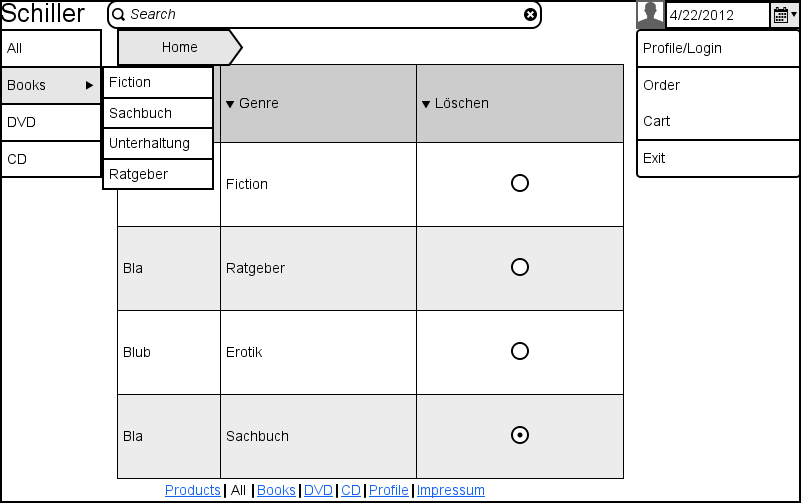
\includegraphics[width=350px]{1Home_Costumer.png}


\subsection{Dialogbeschreibung}

\paragraph{Dieser, für die Dialogübersicht bereits verwendete Dialog ist Startseite eines jeden Nutzer, sowie Artikelübersicht mit Kauffunktion.\\ \\}
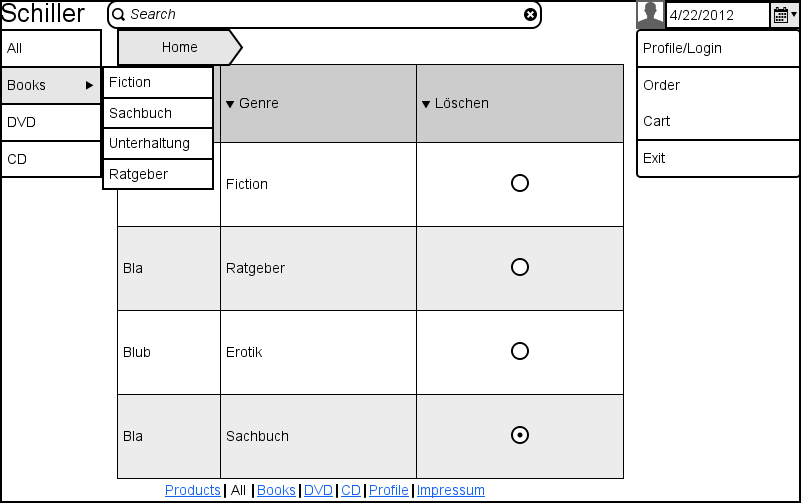
\includegraphics[width=350px]{1Home_Costumer.png}

\paragraph{Die Maske zeigt das Einloggen eines Nutzers. Es enthält auch die Option zur Registrierung eines noch nicht registrierten Nutzers.\\ \\}
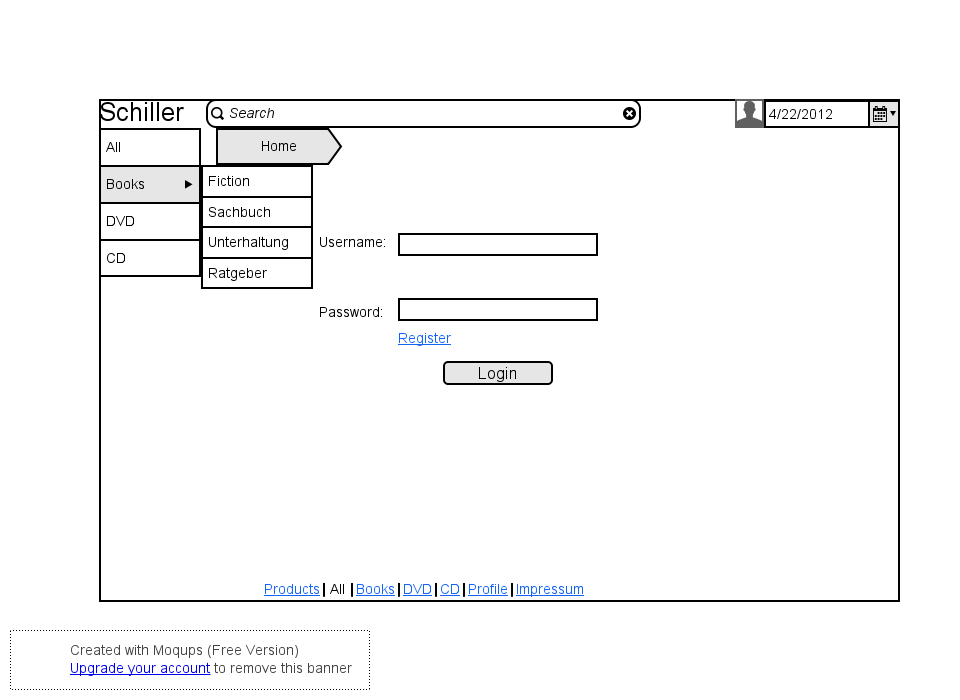
\includegraphics[width=350px]{2Login.png}

\paragraph{Ein Nicht-registrierter Nutzer kann sich über dieses Formular mit einem Klick auf den Knopf Register registrieren, soweit alle Textfelder valide ausgefüllt wurden.\\ \\}
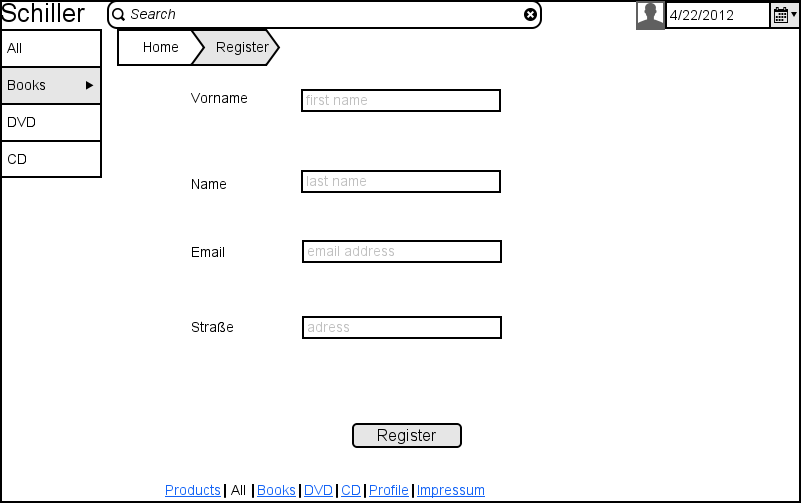
\includegraphics[width=350px]{3Register.png}

\paragraph{Diese Ansicht zeigt die Profilseite eines eingeloggten Kunden. Dieser kann seine angegebenen Daten einsehen und bei Bedarf ändern. Außerdem kann er Rechnungen seiner getätigten Bestellungen einsehen.\\ \\}
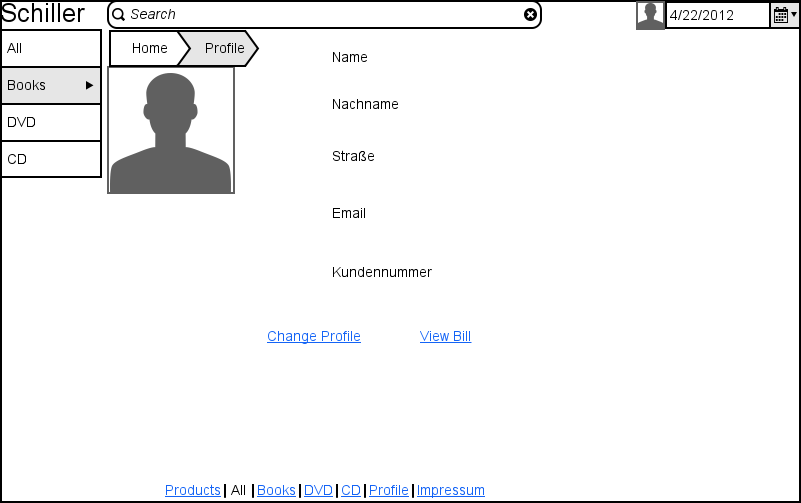
\includegraphics[width=350px]{4ProfileView.png}

\paragraph{Das Layout einer Informationsseite für einen Artikel ist ähnlich der eines Nutzerprofils aufgebaut und zeigt die Attribute eines Artikels. Hier kann man sich auch für den Kauf dieses Artikels entscheiden.\\ \\}
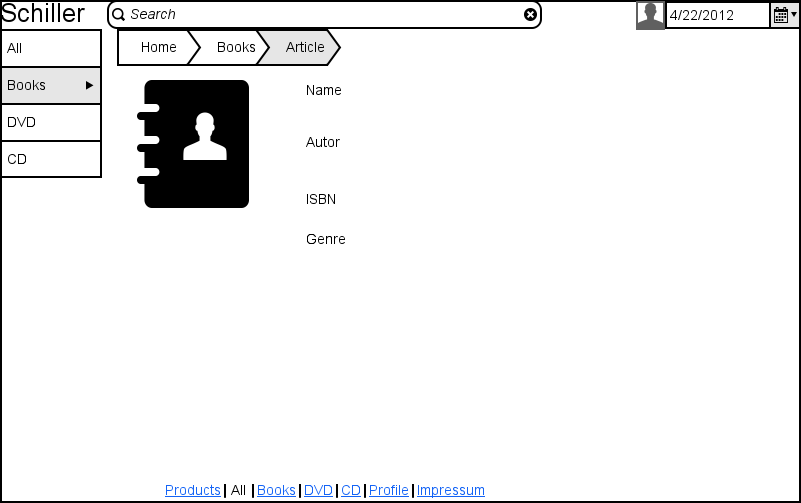
\includegraphics[width=350px]{5ArticleView.png}

\paragraph{Diese Maske bietet die Ansicht des Kalenders. Hier können Veranstaltungstermine eingetragen sein, welche der Kunde einsehen kann.\\ \\}
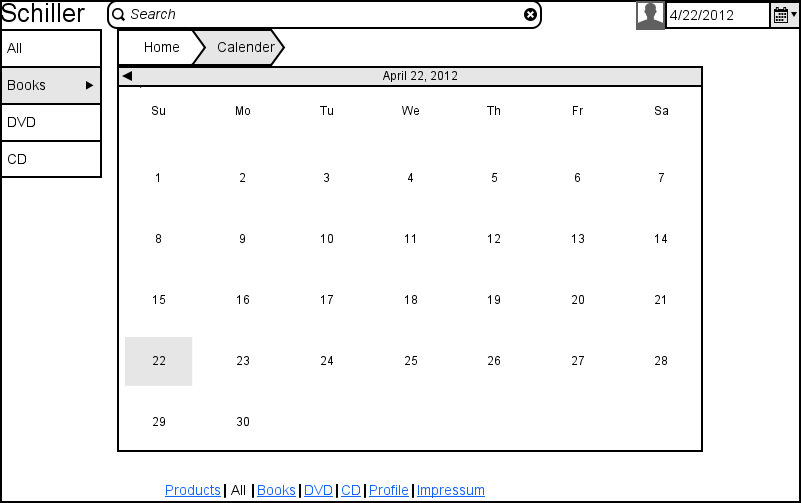
\includegraphics[width=350px]{6CalenderView.png}

\paragraph{Diese Seite zeigt die Artikelsortierung nach dem Artikel Buch spezialisiert, welche durch einen Klick auf die linke Navigationsleiste sortiert wurde. Hier ist es möglich die Bücher in der rechten Tabellenspalte mit einem Klick auf die runden Knöpfe zu selektieren und durch den Knopf kaufen zu der Einkaufswagenansicht mit der Auswahl an Artiken zu wechseln.\\ \\}
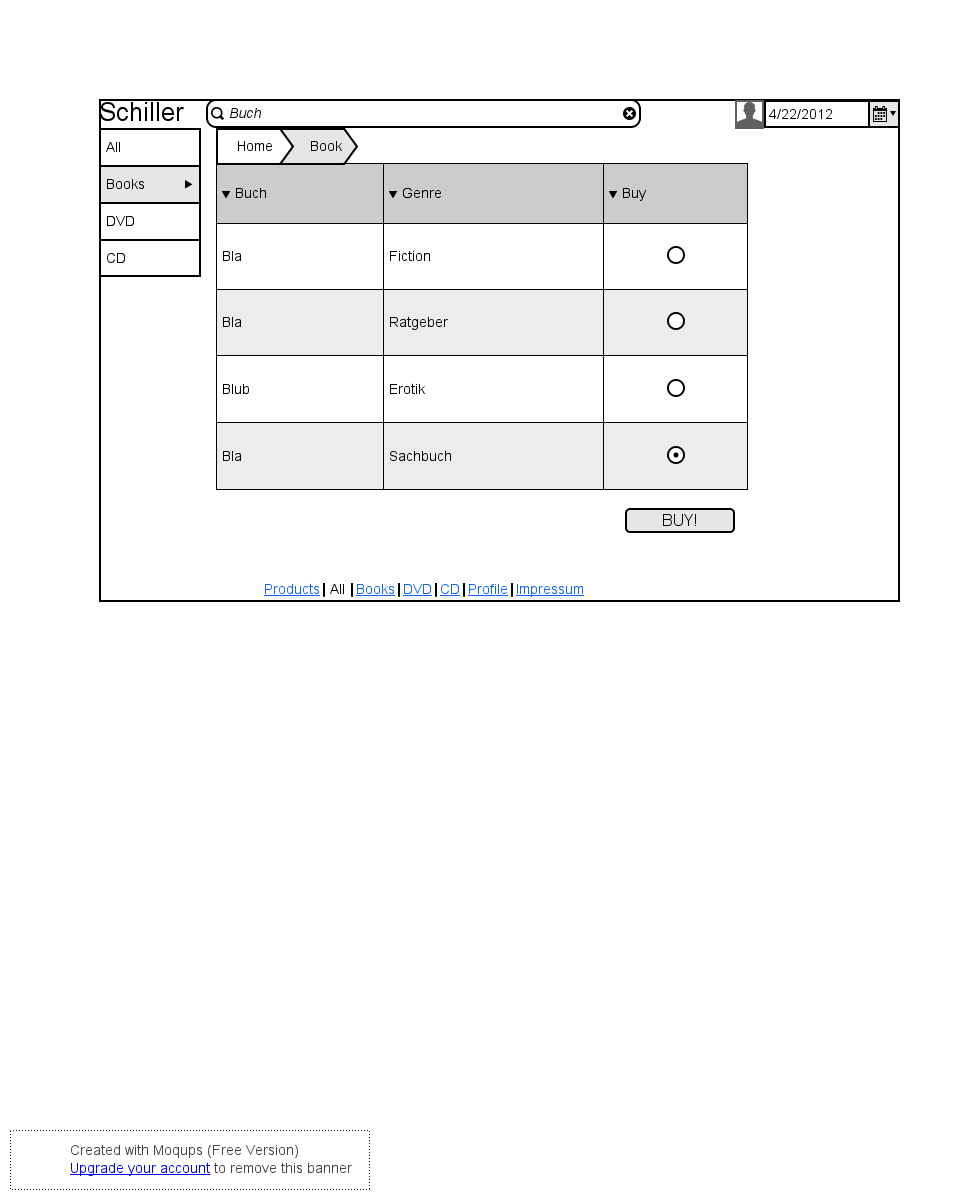
\includegraphics[width=350px]{7bookSearch.png}

\paragraph{Dies ist die Einkaufswagenansicht. Hier kann sich der Kunde über die Auswahl seiner Artikel, welche er im Begriff ist zu kaufen vergewissern. Er kann Artikel nach belieben wieder aus dem Einkaufswagen entfernen, nach dem gleichen Layout, wie er auch Artikel selektieren konnte. Mit einem Klick auf den Checkout Knopf gelangt der Kunde zum Kaufsbildschirm.\\ \\}
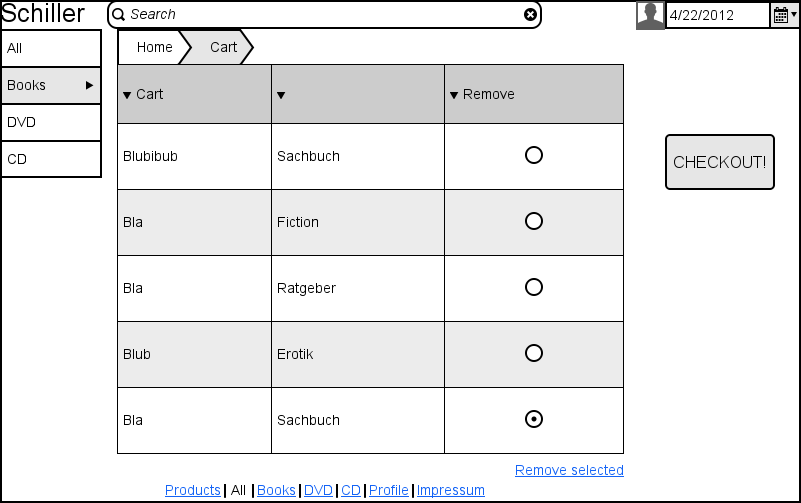
\includegraphics[width=350px]{8CartView.png}

\paragraph{Hier wird eine Übersicht der Informationen angezeigt, die für die Bestellung eines Artikels von nöten sind. Es werden die selektierten Artikel, sowie die Benutzerinformationen angezeigt, an dessen Adresse der Artikel geschickt werden soll. Wenn alles zur Zufriedenheit des Kunden eingetragen ist, kann dieser auf den Buy Knopf klicken, um die Bestellung abzuschließen.\\ \\}
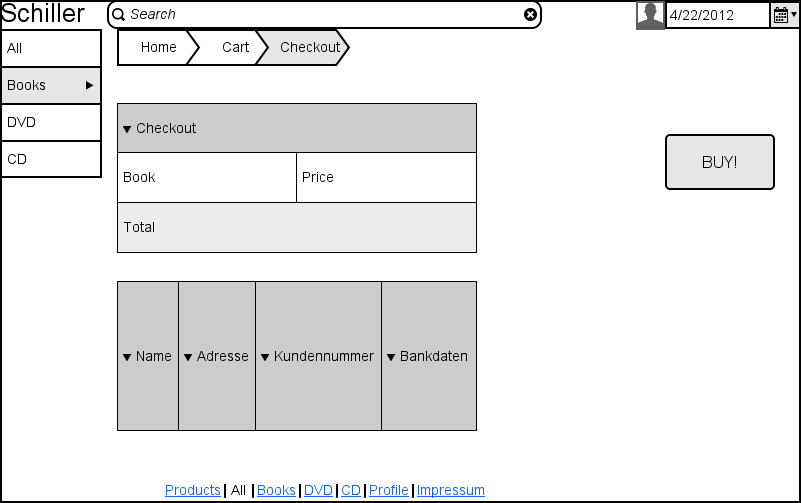
\includegraphics[width=350px]{9CheckOut.png}

\paragraph{Dieser Bildschirm stellt die Bestätigung einer vom Kunden getätigten Bestellung dar. Von diesem Bild aus kann er wieder auf die Bestellungen zugreifen.\\ \\}
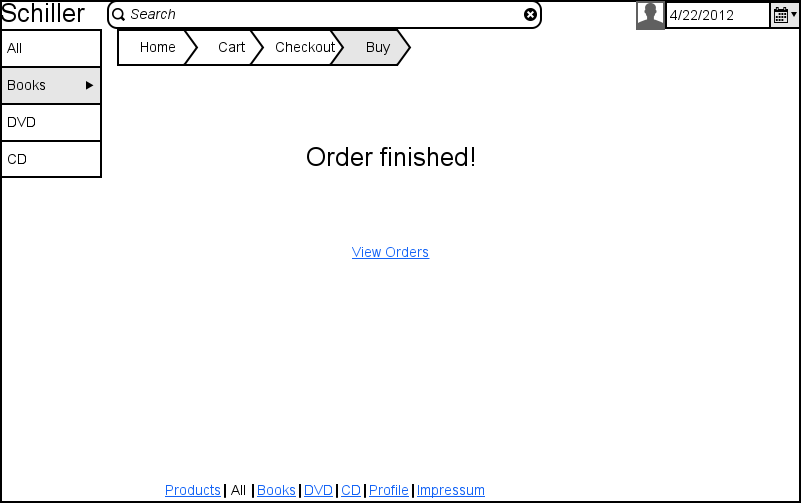
\includegraphics[width=350px]{10SuccessfullyOrdered.png}

\paragraph{Die Einsicht der getätigten Bestellung stellt diese Ansicht dar. Hier kann der Kunde direkt eine Rechnung einsehen und auch die Bestellung wieder stornieren.\\ \\}
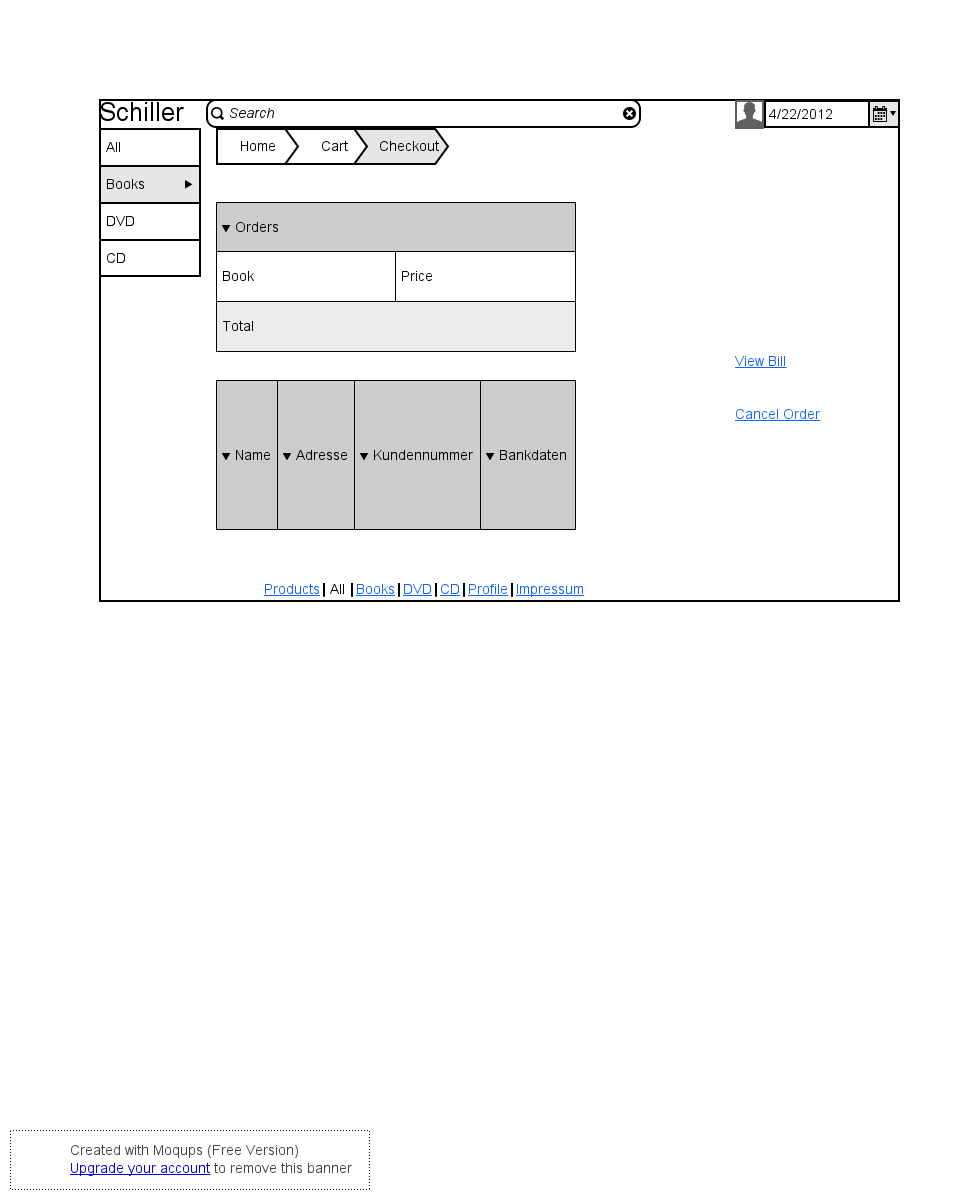
\includegraphics[width=350px]{11OrderView.png}

\paragraph{Diese Maske zeigt die Einsicht einer Rechnung. Der Kunde kann eine Rechnung auch als Dokument anfordern.\\ \\}
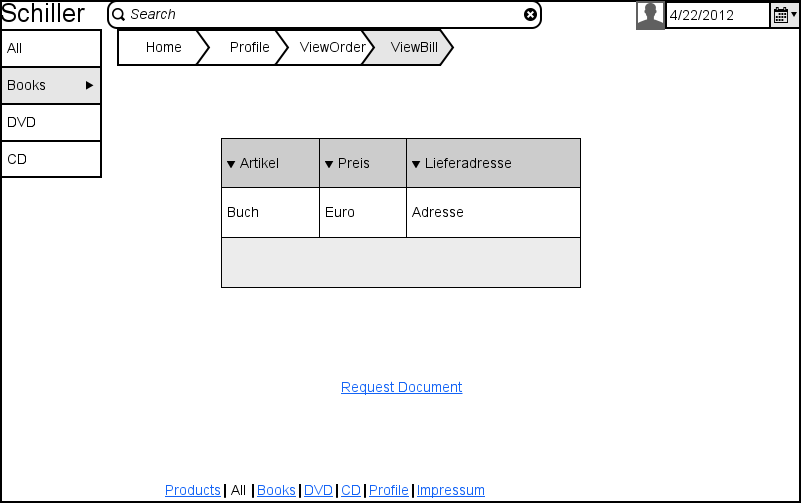
\includegraphics[width=350px]{12BillView.png}

\paragraph{Bei einer Stornierung der Bestellung wird ein letztes zu bestätigendes Bild angezeigt, um eine Bestellung rückgängig zu machen.\\ \\}
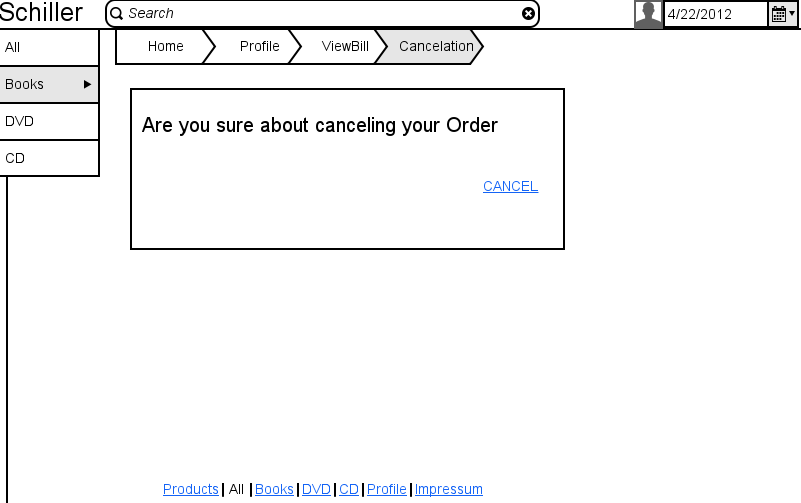
\includegraphics[width=350px]{13Cancelation.png}

\paragraph{Diese Ansicht stellt den üblichen Startbildschirm eines Angestellten dar. Diese unterscheidet sich nur aufgrund der rechten Navigationsleiste grundlegend von der des Kunden bzw. allgemeinen Nutzers. Diese Navigation zeigt die Verwaltungsoptionen, die ein Angestellter angepasst auf seine Rolle bzw. Befugnis ausführen kann.\\
In diesem Beispiel handelt es sich um den Bildschirm eines Artikelverwalters, da auf dieser Seite bereits die Verwaltung der Artikel angedeutet ist.\\ \\}
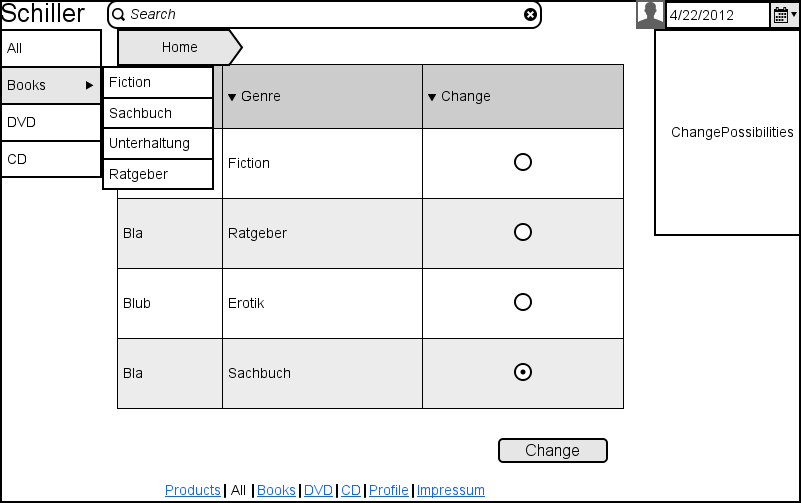
\includegraphics[width=350px]{14Home_Employee.png}

\paragraph{Diese Maske zeigt die Ansicht eines Benutzerverwalters, der nach Profilen suchen, sowie diese verwalten kann.\\ \\}
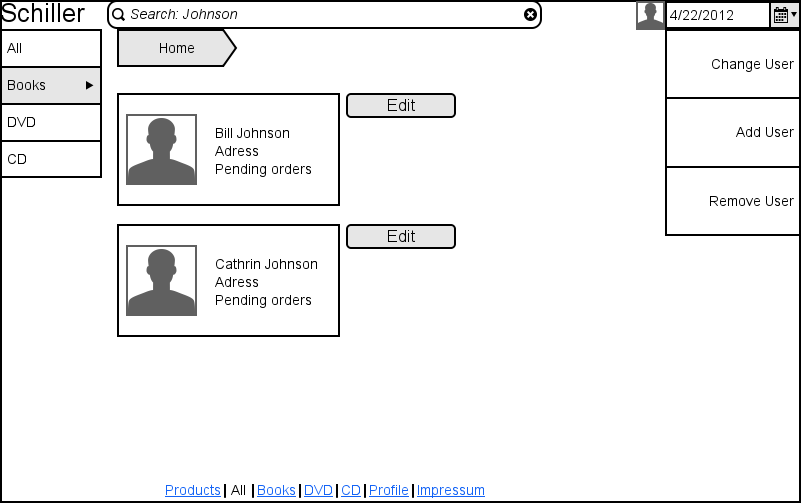
\includegraphics[width=350px]{15ChangeUser.png}

\paragraph{Hier wird die Option eines Artikelverwalters angezeigt, die Genres zu verwalten, die einem Artikel angehören können.\\ \\}
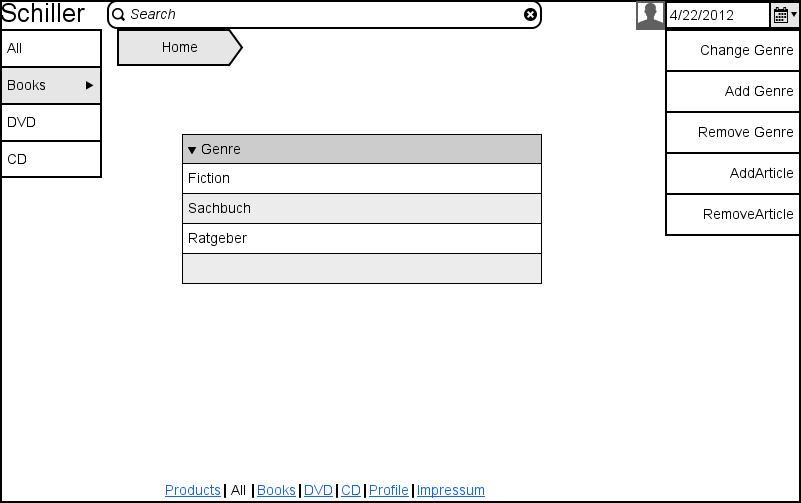
\includegraphics[width=350px]{16ChangeGenre.png}

\paragraph{Das Verwalten eines speziellen Artikels zeigt diese Maske, wieder aus der Sicht eines Artikelverwalters.\\ \\}
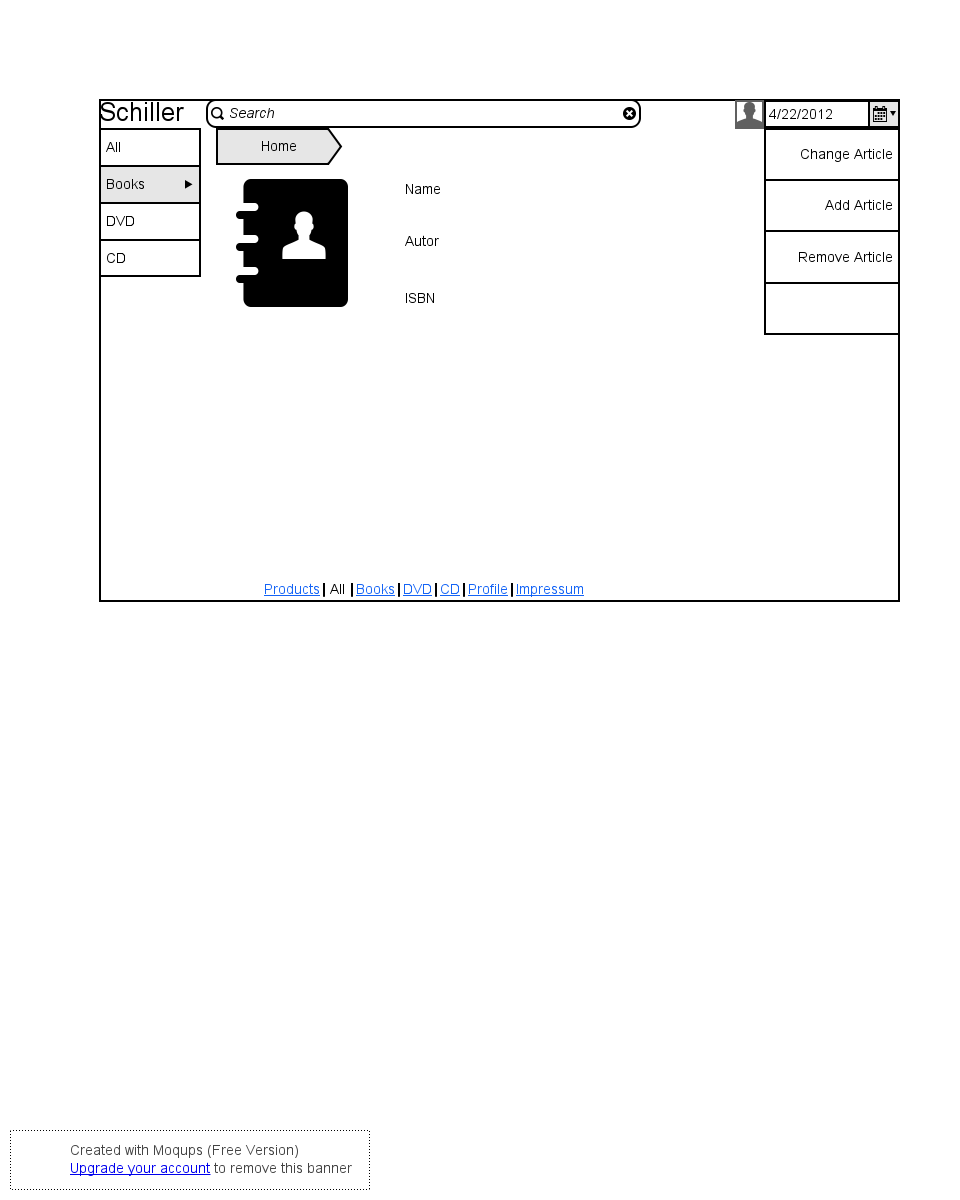
\includegraphics[width=350px]{17ChangeArticle.png}

\paragraph{Der Veranstaltungsverwalter kann in dieser Ansicht Kalender, sowie Veranstaltungen und Räume verwalten.\\ \\}
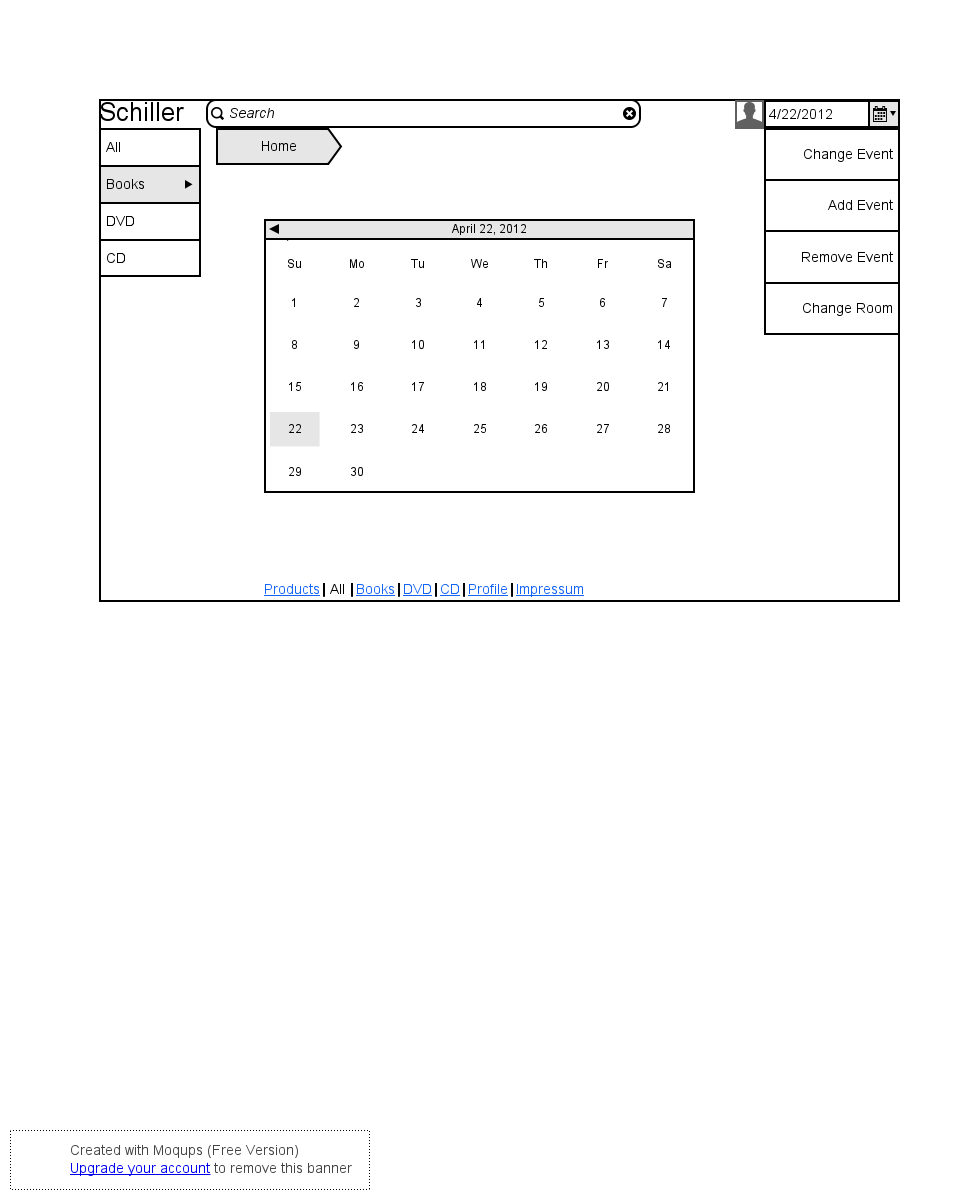
\includegraphics[width=350px]{18ChangeCalender.png}

\paragraph{Zur Raumverwaltung kommt der Veranstaltungsverwalter über die Kalenderverwaltungsansicht. Hier können Räume für Veranstaltungen, sowie für die Buchhandlung im allgemeinen verwaltet werden.\\ \\}
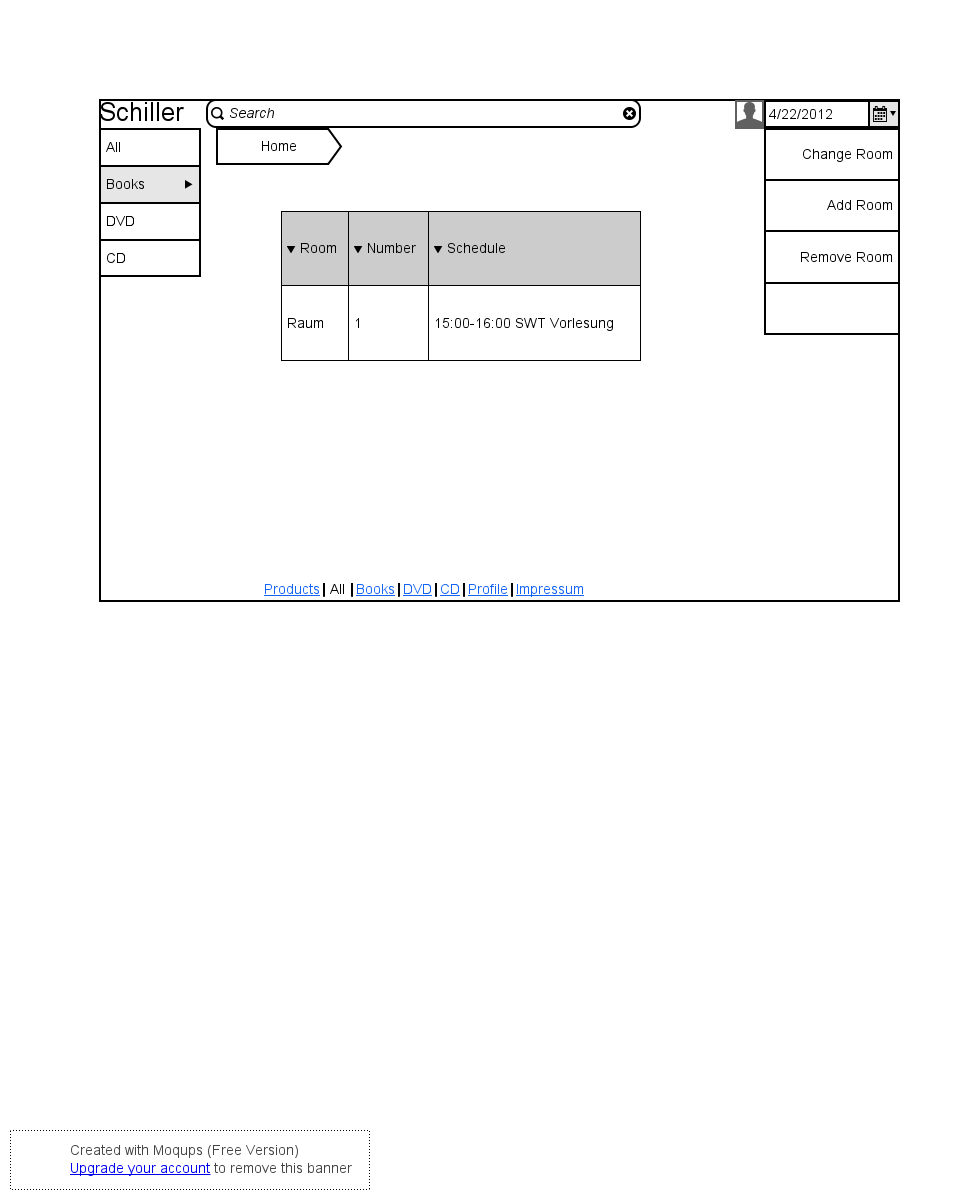
\includegraphics[width=350px]{19ChangeRoom.png}


\section{Datenmodell}

\subsection{Überblick: Klassendiagramm}

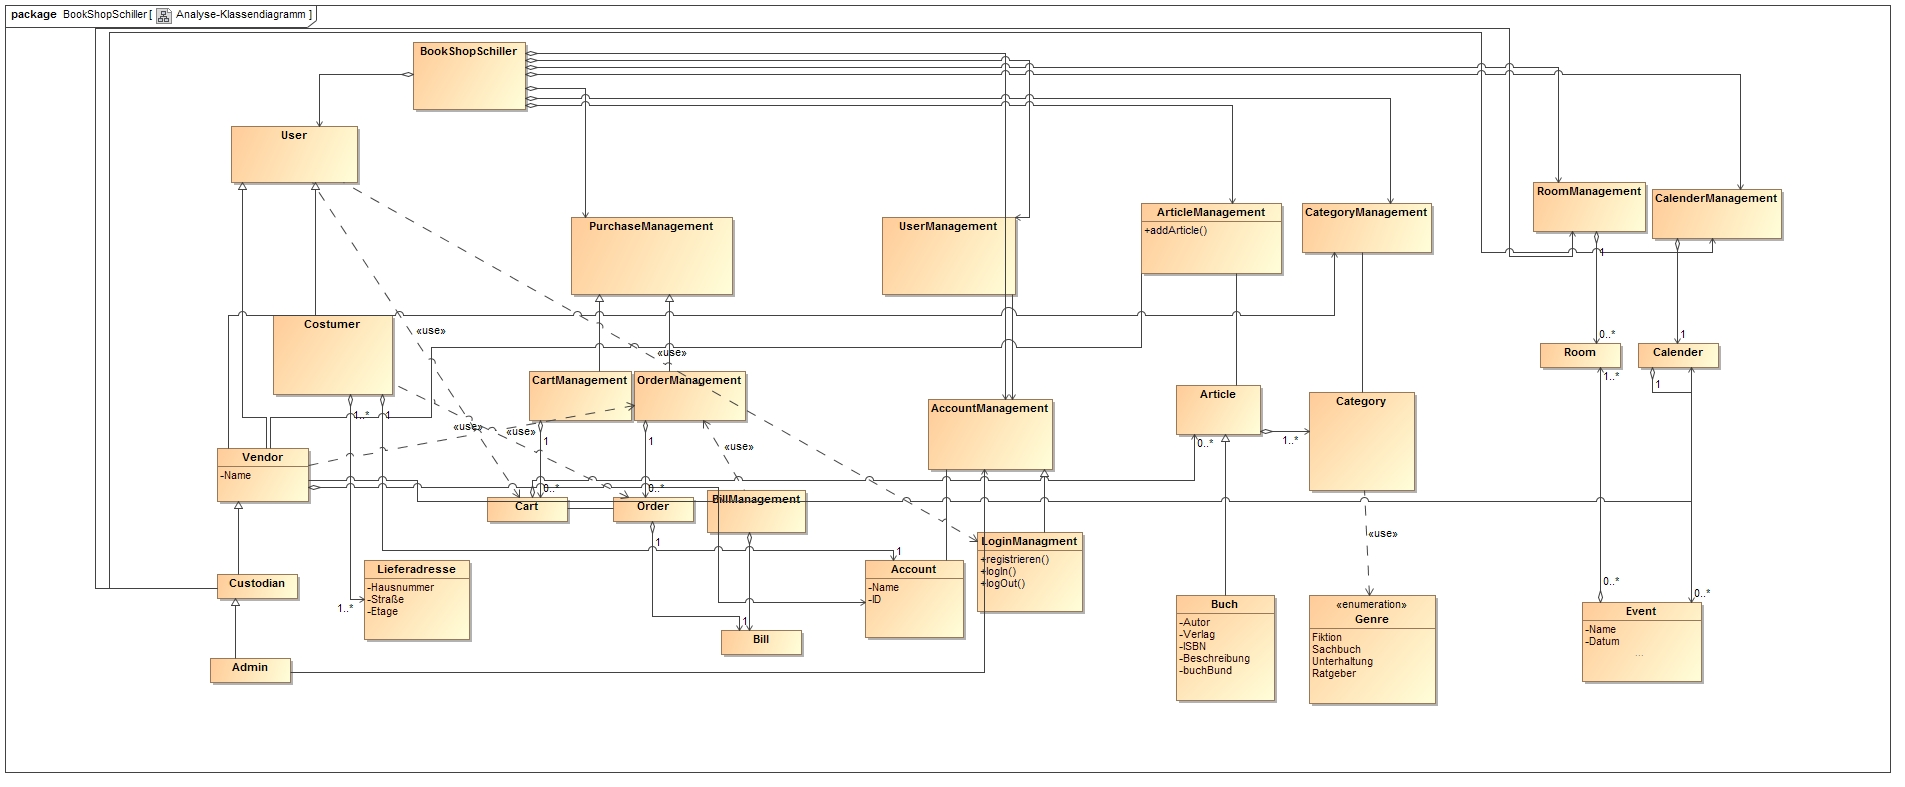
\includegraphics[width=350px]{analyse-klassendiagramm.jpg}

\subsection{Klassen und Enumerationen}

\begin{longtable}{|p{100px}|p{250px}|}
	\hline
	\rowcolor[HTML]{C0C0C0} 
	Klasse/Enumeration & Beschreibung \\ \hline
	BookShopSchiller & Hauptklasse, die alle Funktionen zusammenführt. \\ \hline
	Guest & Klasse für einen  uneingeloggten Benutzer, kann den Einkaufswagen nutzen, sich über das Benutzermanagement einloggen oder kann sich registrieren, kann außerdem die Suchfunktion nutzen. \\ \hline
	Costumer & Klasse für einen eingeloggten Benutzer als Kunde, erbt von dem Guest und kann des weiteren auf sein Konto zugreifen. \\ \hline
	Employee & Klasse für einen Angestellten, erbt ebenfalls von Guest.  \\ \hline
	UserManager & Klasse erbt von Employee und kann außerdem auf die Verwaltung der Profile zugreifen. \\ \hline
	ReadingManager & Klasse erbt von Employee und kann außerdem auf die Verwaltung der Veranstaltungen zugreifen \\ \hline
	SaleManager & Klasse erbt von Employee und kann außerdem auf die Verwaltung der Bestellungen zugreifen. \\ \hline
	ArticleManager & Klasse erbt von Employee und kann außerdem auf die Verwaltung der Artikel zugreifen. \\ \hline
	Admin & Klasse erbt von den „Manager“-Klassen, um Gewalt über alle Funktionalitäten zu haben. \\ \hline
	Chef & Klasse erbt von Employee und kann außerdem Einsicht in die finanziellen Bilanzen bekommen. \\ \hline
	Lieferadresse & Enumeration gehört zu jedem Costumer. Sie enthält die Daten eines Kunden(Hausnummer, Straße, Etage) \\ \hline
	SaleManagement & Ist die Oberklasse zur Verwaltung/Funktionalität des Verkaufs. Sie regelt daher den Verkauf an Kunden. Der SaleManager benutzt die Funktionalitäten dieser Klasse. \\ \hline
	CartManagement & Klasse kümmert sich um die Verwaltung des Einkaufswagen durch einen Costumer. \\ \hline
	OrderManagement & Klasse verwaltet und bietet die Funktionalitäten einer jeden Bestellung. \\ \hline
	BalanceSheet & Klasse bietet Funktionalitäten zum Einsehen der Ein- und Ausgaben. Enthält Werte für Einkommen und Ausgaben und die Berechnung einer Bilanz. \\ \hline
	Cart & Klasse stellt die Umsetzung eines Einkaufswagens dar. \\ \hline
	Order & Klasse stellt die Umsetzung einer Bestellung dar. \\ \hline
	BillViewer & Klasse liefert die Funktionalitäten des Einsehens einer Rechnung für den Kunden \\ \hline
	Bill & Klasse stellt die Umsetzung einer Rechnung dar. \\ \hline
	Account	 & Klasse stellt die Umsetzung eines Personenkontos dar. \\ \hline
	UserManagement  & Ist die Oberklasse zur Verwaltung/Funktionalität des Profils/Kontos. Sie regelt also das Interagieren mit dem Account für den Kunden. Der UserManager benutzt die Funktionalitäten dieser Klasse \\ \hline
	ProfileManagement & Klasse verwaltet die Profile und bietet Funktionalitäten für jeden Nutzer. \\ \hline
	RegisterManagement & Klasse bietet Funktionalitäten zum Registrieren eines jeden Nutzers. \\ \hline
	ProfileViewer & Klasse liefert Funktionalitäten des Einsehens eines Profils für den Benutzer. \\ \hline
	LogInOut & Klasse kümmert sich um die Funktionen des Ein- und Ausloggens. \\ \hline
	ArticleManagement & Die Oberklasse bietet Funktionalitäten zur Verwaltung sämtlicher Artikel. Diese bietet Funktionalitäten zum Durchsuchen der Artikelbestände, sowie zum verwalten dieser. Sie wird vom ArticleManager benutzt. \\ \hline
	CategoryManagement & Klasse kümmert sich um die Kategorisierungs-/Verwaltungsfunktionalitäten jeglicher Artikel. \\ \hline
	BookManagement & Klasse erbt von ArticleManagement und  bietet  Kategorisierungs-/Verwaltungsfunktionalitäten von Büchern \\ \hline
	DVDManagement & Klasse erbt von ArticleManagement und  bietet  Kategorisierungs-/Verwaltungsfunktionalitäten von DVDs \\ \hline
	CDManagement & Klasse erbt von ArticleManagement und  bietet  Kategorisierungs-/Verwaltungsfunktionalitäten von CDs \\ \hline
	Storage & Klasse stellt Umsetzung eines Lagers dar. \\ \hline
	ArticleViewer & Klasse liefert Funktionalitäten zum Anzeigen eines jeden Artikels. \\ \hline
	BookViewer & Klasse erbt von ArticleViewer und liefert Funktionalitäten zum Anzeigen eines Buches. \\ \hline
	DVDViewer & Klasse erbt von ArticleViewer und liefert Funktionalitäten zum Anzeigen einer DVD. \\ \hline
	CDViewer & Klasse erbt von ArticleViewer und liefert Funktionalitäten zum Anzeigen einer CD. \\ \hline
	Article & Klasse stellt die Umsetzung eines Artikels dar. Enthält Werte für den Titel, Cover und eine Beschreibung. \\ \hline
	Category & Klasse stellt die Umsetzung einer Kategorie dar. \\ \hline
	Book & Klasse erbt von Article und stellt die Umsetzung eines Buches dar. Enthält Werte für den Autor, Verlag und die ISBN-Nummer. \\ \hline
	DVD & Klasse erbt von Article und stellt die Umsetzung einer DVD dar. Enthält Werte für Regisseur \\ \hline
	CD & Klasse erbt von Article und stellt die Umsetzung einer CD dar. Enthält Werte für Interpret. \\ \hline
	Genre <Enumeration> & Enumeration ist Teil einer Kategorienklasse und listet alle Genres auf. Enthält die Werte Fiktion, Sachbuch, Unterhaltung, Ratgeber. \\ \hline
	ReadingManagement & Oberklasse bietet Funktionalitäten zur Verwaltung und Einsicht von Veranstaltungen. \\ \hline
	RoomManagement & Klasse kümmert sich um die Verwaltung von Räumlichkeiten. \\ \hline
	CalenderManagement & Klasse verwaltet die Organisation von Veranstaltungen in einem Kalender. \\ \hline
	CalenderViewer & Klasse liefert Einsicht in den Kalender für alle Nutzer \\ \hline
	Room & Klasse stellt die Umsetzung eines Raumes dar. Enthält Werte für Namen und Nummer des Raumes. \\ \hline
	Calender & Klasse stellt die Umsetzung eines Kalenders dar. \\ \hline
	Event & Klasse stellt die Umsetzung einer Veranstaltung dar. Enthält Werte für Namen der Veranstaltung und dessen Datum. \\ \hline
\end{longtable}


\section{Akzeptanzfälle}

\begin{longtable}{|p{50px}|p{250px}|p{50px}|}
	\hline
	\rowcolor[HTML]{C0C0C0} 
	Test Case ID & Beschreibung & Ergebnis \\ \hline
	TC00000 & Try to change anything without proper permissions & Fail \\ \hline
	TCUC011 & Wrong Username & Login Fail \\ \hline
	TCUC012 & Wrong Password & Login Fail \\ \hline
	TCUC021 & E-Mail Adress format wrong & Reenter E-Mail \\ \hline
	TCUC022 & Username already in use & new username \\ \hline
	TCUC031 & delete last admin & Fail \\ \hline
	TCUC061 & user not existing & no result \\ \hline
	TCUC091 & Category not found & no result \\ \hline
	TCUC131 & checkout as guest & redirect to login \\ \hline
	TCUC191 & place reading in same room and time & fail \\ \hline
	TCUC201 & create similiar rooms & fail \\ \hline
\end{longtable}

\section{Offene Punkte}

\begin{itemize}
	\item GUI
	\item Akzeptanzfälle
\end{itemize}

\end{document}